\chapter{Terrain Generation by Simulated Erosion}
\label{chapter:ErosionSimulation}



% FOOTNOTE THE ATTRIBUTIONS
\let\thefootnote\relax\footnote{Portions of this chapter previously appeared as: FIX \bibentry{Chen:2010:QAS:1869790.1869867} }

\let\thefootnote\relax\footnote{Portions of this chapter previously appeared as: FIX \bibentry{Kamalzare-ValidationOfErosionModeling} }





Understanding the evolution of terrain requires a firm grasp on the erosion processes that contribute to the formation of it. To that end, and motivated by the devastation of Hurricane Katrina in 2005, 
my research group
% the levee research group at Rensselaer Polytechnic Institute
has
% , over the last several years, 
developed a hydraulic erosion computer simulation coupled with a fluid simulation, as well as conducted several laboratory experiments of levee overtopping. 
These experiments are described in detail by Kalamzare et al. \cite{Kamalzare-ValidationOfErosionModeling} and Gross et al. \cite{gross_icse_2010}.
In addition to providing valuable insight into the propagation of erosion over a levee surface, the laboratory experiments also provide a source for validation of the erosion simulation. 
This chapter will discuss my contributions to this work, and analyze some of its results.

The simulation focuses on small-scale erosion, or the formation of channels along the downslope of a levee. A levee has the structure seen in Figure \ref{figure:levee_diagram}. There are five sections of the levee geometry: the source, upslope, crest, downslope, and sink. The dimensions seen in the figure refer to the small scale levee models used in laboratory experiments. Each pair of sections is divided by a letter, A, B, C, or D. The source and upslope sections are known as the levee's \emph{wet side}, as this is the side that is generally facing the body of water the levee is providing protection from. The crest is the tallest section of the levee, the long and flat area that generally prevents levees from failing. As long as the crest and downslope remain dry, the levee is in no danger of failing. 

However, in overtopping conditions, during which water flows over the crest of the levee and down the downslope in large quantities, the downslope and crest can erode away. This is the time of breach of the levee. Fread \cite{DAMBRK_REPORT}, from the National Weather Service, defined time to breach as the duration of time between the initial formation of a channel and the time at which the channel has reached the upslope of the levee, forming a clear channel along which breaching water runs. Once a levee is breached, its failure is imminent. 

The project's coupled fluid and erosion simulations, designed to study small-scale erosion processes, are described in detail by Chen et al. \cite{chen-geo-frontiers-2011}. The simulation uses the SPH system and is based on the work of M\"{u}ller et al. \cite{Muller-Particle} for the simulation and the physical erosion model presented by Briaud \cite{Briaud-ErosionByOvertopping}. 
% % This chapter shall describe, in detail, the laboratory experimentation, followed by a chapter outlining the simulation implementation phase of the project, including analysis of a series of results.


% \section{Laboratory Experimentation}
% \label{section:LaboratoryExperimentation}
% 
% 
% \begin{figure*}[t]
% \centering
% \begin{minipage}[b]{0.9\linewidth}
% \begin{center}
% 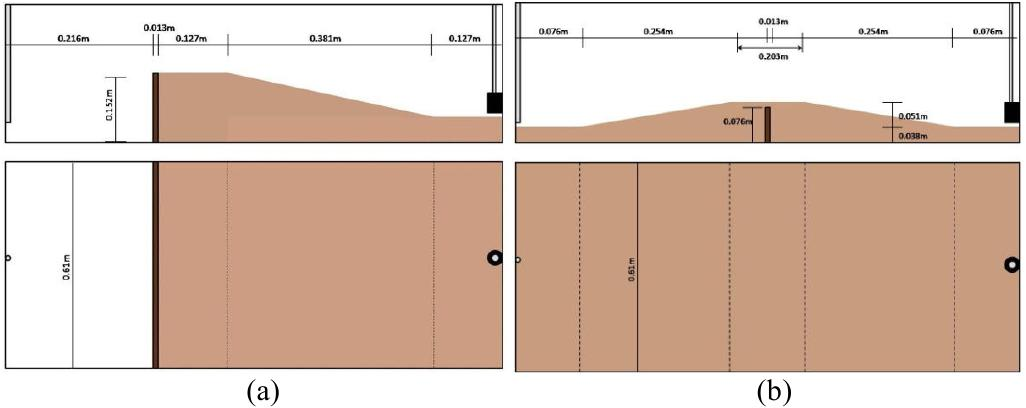
\includegraphics[width=\textwidth]{images/LabExperimentSetupSchematic.jpg}
% \end{center}
% \end{minipage}
% \caption[Laboratory experiment setup schematic]
% {\label{figure:LaboratorySetupSchematic} A schematic view of both the a) half-levee and b) full-levee experiment test setup. The upper images are section views, while the lower images are the setup plan. }
% \end{figure*}
% 
% 
% \begin{figure}[t]
%   \centering
%   \begin{minipage}{0.98\linewidth}
%   \begin{minipage}{0.355\textwidth}
%     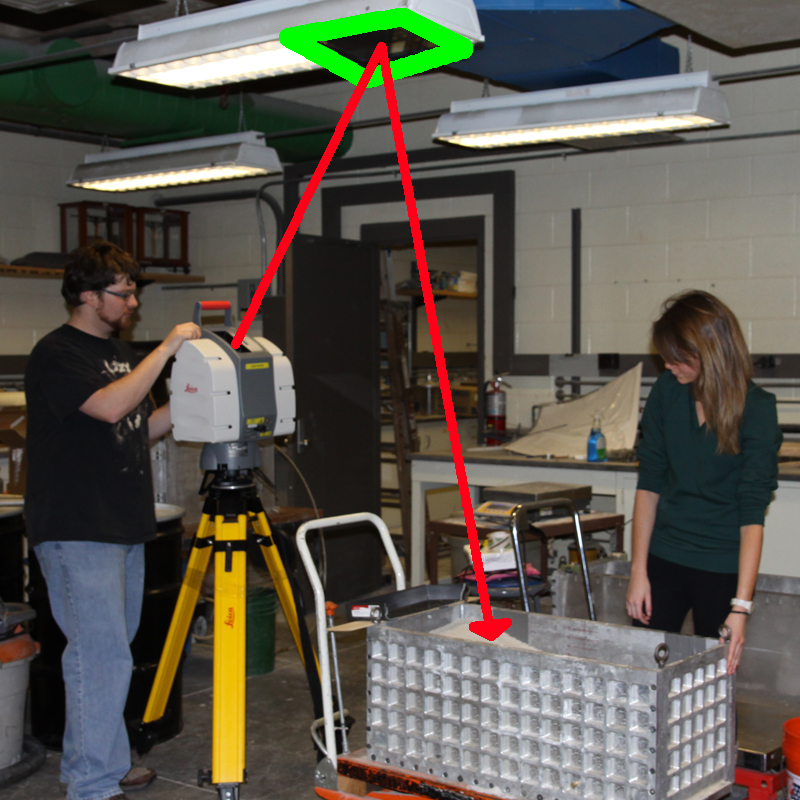
\includegraphics[width=\textwidth]{images/scanner_setup_small_annotated.jpg}
%   \end{minipage}
%   \begin{minipage}{0.635\textwidth}
%     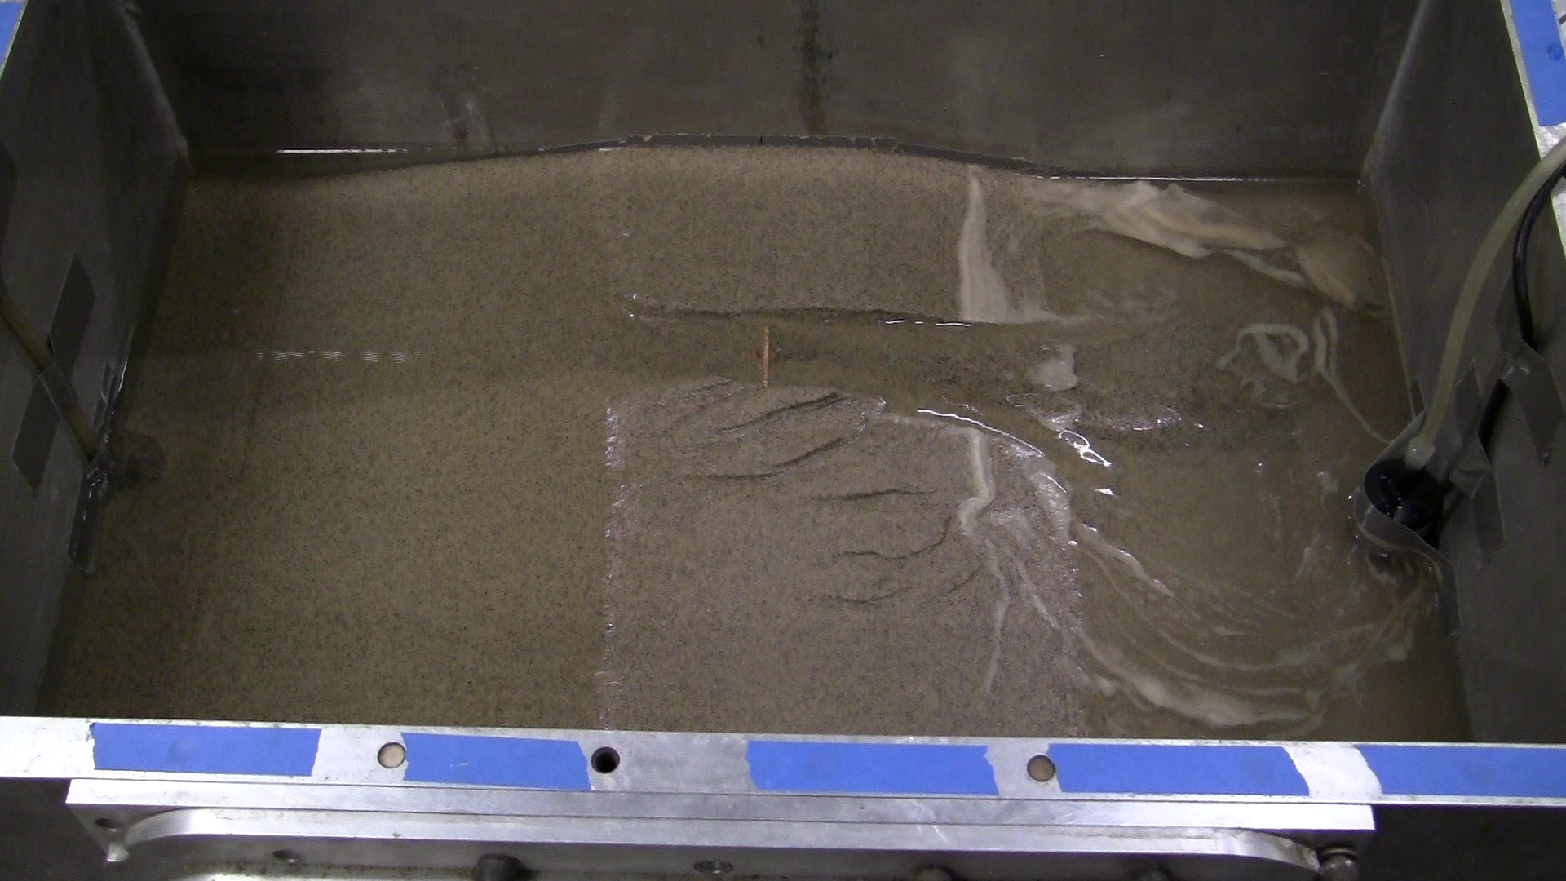
\includegraphics[width=\textwidth]{images/sand-10mins-phy-test.png}
%   \end{minipage}
%   \end{minipage}
%   \caption[Experimental setup of real world experiments]{\label{figure:1GExperiments} Left: LIDAR scanner setup, where LIDAR beams are shot off of a mirror placed on the ceiling and hit the surface of the levee model. Right: An image from the 1-g experiment, in which water flows left to right. A deep channel has clearly formed along the down slope of the levee model.}
% \end{figure}
% 
% Preparatory 1-g erosion tests were conducted in a laboratory, overtopping tests run on half-levee and full-levee models. A schematic of the setup is shown in Figure \ref{figure:LaboratorySetupSchematic}. For the half-levees, the embankment was anchored at one end by a $\frac{1}{2}$ inch thick piece of plywood sealed to the bottom of the tank using silicone. The plywood was 6'' high and 24'' wide. The box was 14'' x 24'' x 36'', and the plywood separated the water source from the embankment crest. For the half-levee tests, the plywood formed the source reservoir, which created rising water that overtopped the embankment crest, and its dimensions were 6'' x 24'' x 8.5''. For the full-levee tests, water was allowed to fill the wet side portion of the levee, allowing natural overtopping.
% 
% The embankment was made of well-graded medium sand, created from \emph{lifts}. A lift is a thin layer of sand piled onto a compacted layer. To form the embankment, a 3'' high layer of sand was compacted using a 4'' by 4'' wooden hand tamp, spread a lift over it, and compacted again. The 5:1 embankment measured 5'' at the crest and 15.3'' from crest to toe. A 5'' x 24'' \emph{floodplain} was left at the toe of the embankment to collect the overtopping water with a small aquarium pump, placed $\frac{1}{2}$'' above the floodplain. 
% 
% Water was run over the embankment with a flow rate of 11.1 $\frac{mL}{sec}$. During the course of the test, the formation of rills and gullies is closely observed. An image of the test being run can be see in Figure \ref{figure:1GExperiments}.

% These experiments are described in further detail by Kalamzare et al. \cite{Kamalzare-ValidationOfErosionModeling} and Gross et al. \cite{gross_icse_2010}.

\section{Data Collection}

Layer surface data is collected in the form of a point cloud via a 3D laser range scanner. This 3D point data is then run through a data preparation script that, for each scan, registers the points. It then aligns them to a regular grid in the XY plane, retaining the height values of the points, The points in a grid space have their heights averaged to acquire a single value to use in the data structure. If there are multiple soil layers in a single model, this procedure can be repeated for each one (as they are being assembled), generating a layered data structure. The end result is a grid in which each cell contains an array of soil layers with heights and depths. This data is then loaded in to the Segmented Height Field.

Data collected from the LIDAR scanner can be seen in Figure \ref{figure:LIDARResults}. From each of the cardinal directions around the experiment, a fine resolution scan is taken to obtain as much surface detail as possible. This scan usually has 1mm resolution. From at least two perspectives, a coarse resolution scan (10mm) is taken of the entire room, The coarse resolution scans aid in registration, as they add keypoints for registration algorithms to pick up and use when attempting to transform the data into the same coordinate system. Registration of the data is necessary because of the nature of the equipment. The LIDAR scanner is more mobile than the experimental setup, and thus can be moved around the room to acquire data from different angles. From any one angle, it is impossible to see all of the surface data, and so taking scans from several angles is necessary.

\begin{figure*}[t]
\centering
\begin{minipage}{0.45\linewidth}
\begin{center}
\includegraphics[width=\textwidth]{images/DataScreenshot_BirdsEyeView.jpg}
\end{center}
\end{minipage}
\begin{minipage}{0.45\linewidth}
\begin{center}
\includegraphics[width=\textwidth]{images/DataScreenshot_Scanner_POV.jpg}
\end{center}
\end{minipage}
\caption[Data from the laboratory experiments, scanned with a LIDAR scanner]
{\label{figure:LIDARResults} Two separate LIDAR scans of the laboratory setup. The view on the left is a coarse resolution (\~10mm) scan of the room in which the experiment takes place. The view on the left is a fine resolution (\~1mm) scan of the experimental setup itself. The coarse scan is used for registration purposes, whereas data is taken from the fine resolution  scan.}
\end{figure*}

From the fine resolution scans, the surface points are cropped out. They are then axis-aligned, and can be converted into a data format recognizable by the erosion simulation via the data preparation script described above.
%  From this data format, it can be fed into the erosion simulation.

% \fbox{More here? Better images?}





% The data collected from the laboratory experiments described in Chapter \ref{chapter:ErosionModeling} provided a baseline for comparison for a detailed and accurate erosion simulation.
% 
% % \section{Terrain Representations}



\section{Segmented Height Field (Volumetric Representation)}
\label{section:ErosionSimulationVolumetricTerrainRepresentation}

% Traditionally, terrains are represented by a matrix of elevations, or heightfield, and stored in a Digital Elevation Map (DEM) format, as discussed in Chapter \ref{chapter:TerrainRepresentations}. Other popular representations include voxel grids, particles, and layered height fields. 
This thesis presents a new volumetric representation of terrain data, the Segmented Height Field (SHF), shown schematically in Figure \ref{figure:SHFAbstract}.  It is similar to the layered height field, described in Section \ref{section:VolumetricRepresentations}, in that it is a grid of cells, and each cell contains a list of the layers of soil found in that column. In the SHF, each cell (referred to as a \textit{column}) contains a list of soil \textit{segments} (a rectilinear block of soil).  Segments of the same soil type in adjacent grid columns that have overlapping intervals in height create a \textit{layer}.

\begin{figure*}[t]
\begin{minipage}[b]{0.9\linewidth}
\begin{center}
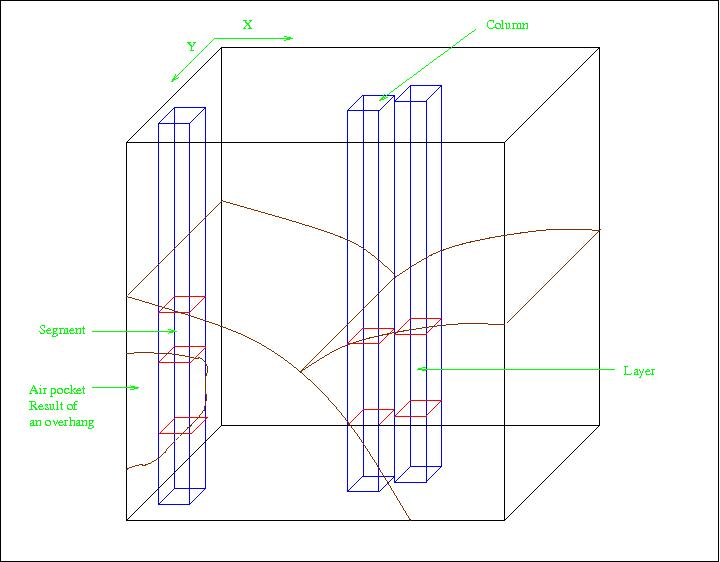
\includegraphics[width=\textwidth]{images/SegmentedHeightField_Schematic.jpg}
\end{center}
\end{minipage}
\caption[Abstract schematic of the Segmented Height Field (SHF)]
{\label{figure:SHFAbstract} A schematic representation of the Segmented Height Field (SHF), as it pertains to multi-layered soil geometry. In the SHF, columns of segments are arranged in a grid. These segments can include air (as noted by the air pocket), and two or more neighboring segments of the same material are referred to as a layer. With these designations, multiple layered soil volumes may be represented. }
\end{figure*}

Several important differences exist between the layered height field and the SHF.  First, SHF allows for layers to be dynamically added and removed throughout the simulation, making accurate re-deposition significantly easier. It is not possible to tell \textit{a priori} where sediment will land and where new layers will have to be added on top of existing ones, so defining the soil layers before the simulation starts is impractical. Second, a layered height field does not allow for two layers of the same soil type to exist in the same list in one grid cell, whereas in the SHF these layers are added automatically. Because there are no restrictions with regards to a soil segment's location within the column SHF naturally supports overhangs and air pockets, which can be modeled either implicitly by gaps in data or explicitly as air layers.

Furthermore, each SHF segment can have spatially varying soil parameters; for example, moisture content. Yet the SHF retains a key advantage of height fields: the layer height is not limited in elevation resolution as it is for a voxel grid. Finally, the SHF can be more memory efficient than either a voxel grid or a layered height field. Voxel grids store redundant data when representing layers that are thick relative to the underlying grid. And, layered height fields are inefficient for accurate representation of complex soil re-deposition, because the addition of new layers is global rather than local. An example of the SHF representing a levee with with three layers can be seen in Figure \ref{figure:SHFDrawn}.

\begin{figure*}[t]
\begin{minipage}[b]{0.9\linewidth}
\begin{center}
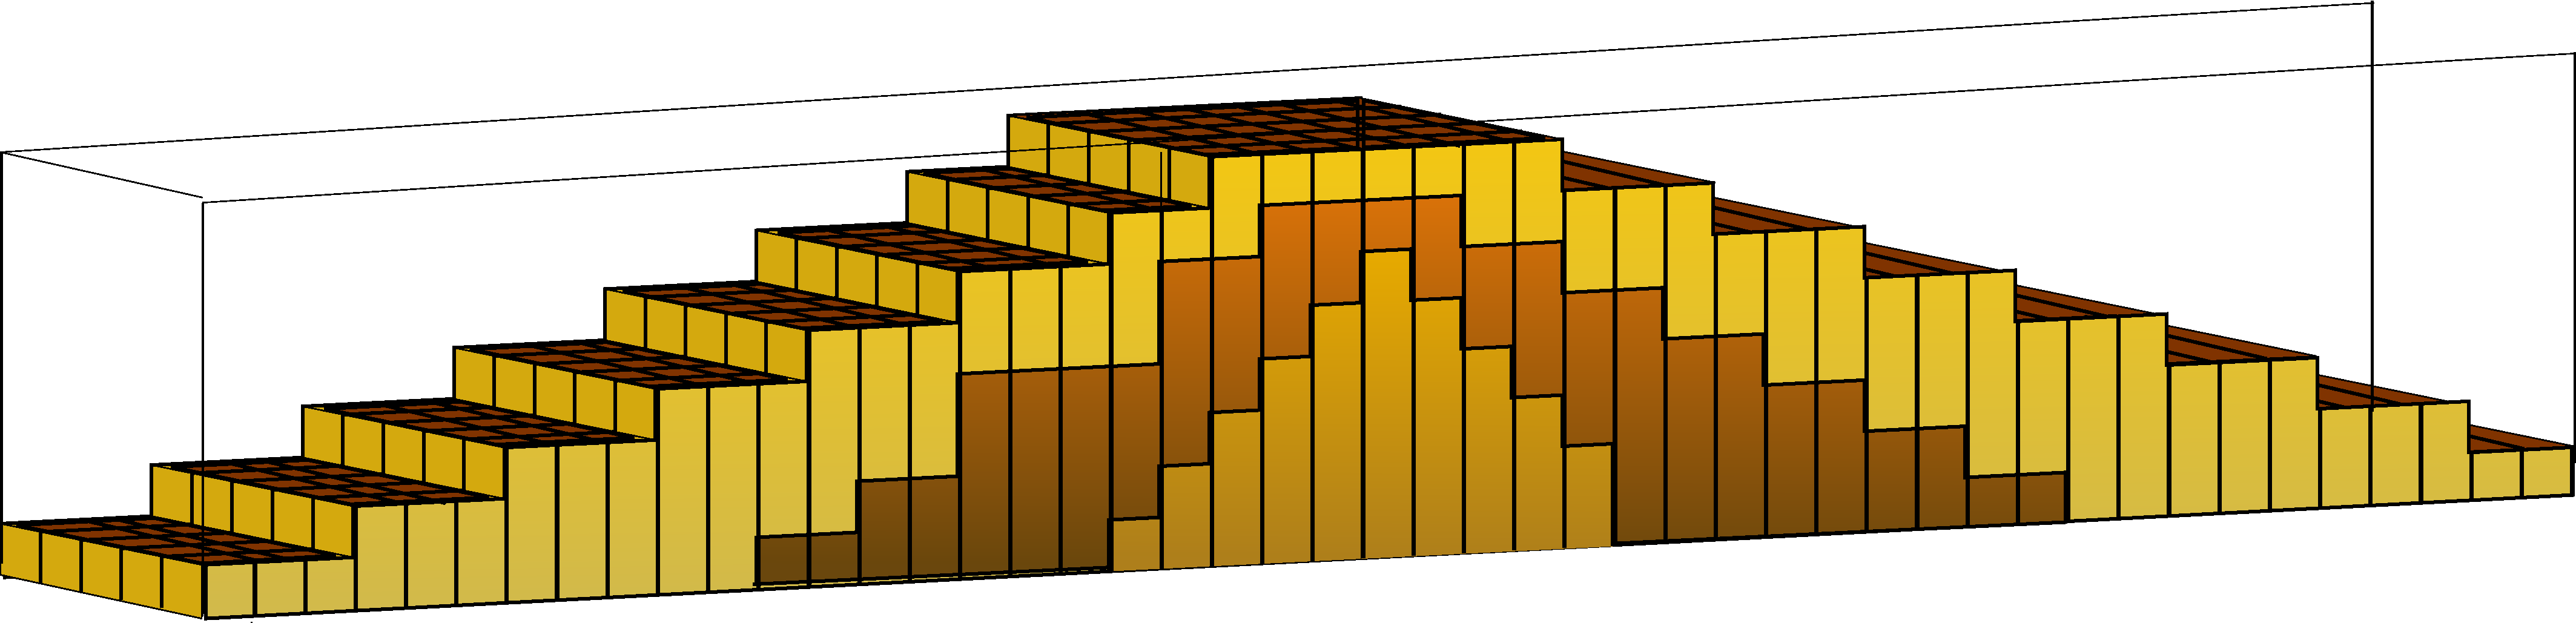
\includegraphics[width=\textwidth]{images/SHF.pdf}
\end{center}
\end{minipage}
\caption[Multi-layered levee-shaped SHF]
{\label{figure:SHFDrawn} A SHF representing a multi-layered levee.}
\end{figure*}



\subsection{Implementation Details}

The SHF is stored as a grid of lists of segments. Each segment is defined by its eight corner points, and the type of material of which it is composed. The material stores all of its necessary properties (such as erodibility), and the segment 
% can 
stores information specific to its volume, mainly the material itself and the coordinates of the corners.
The points designating the eight corner points of the segment are stored in a single master list, in which duplicates (within a very small distance tolerance) are combined. When a segment's corner is a point already in the list, then the segment is assigned the index of the previously stored point instead of creating a duplicate. These points are visualized in Figure \ref{figure:SegmentEdgesAndCornerPoints}.

\begin{figure*}[t]
\centering
\begin{minipage}[b]{0.6\linewidth}
\begin{center}
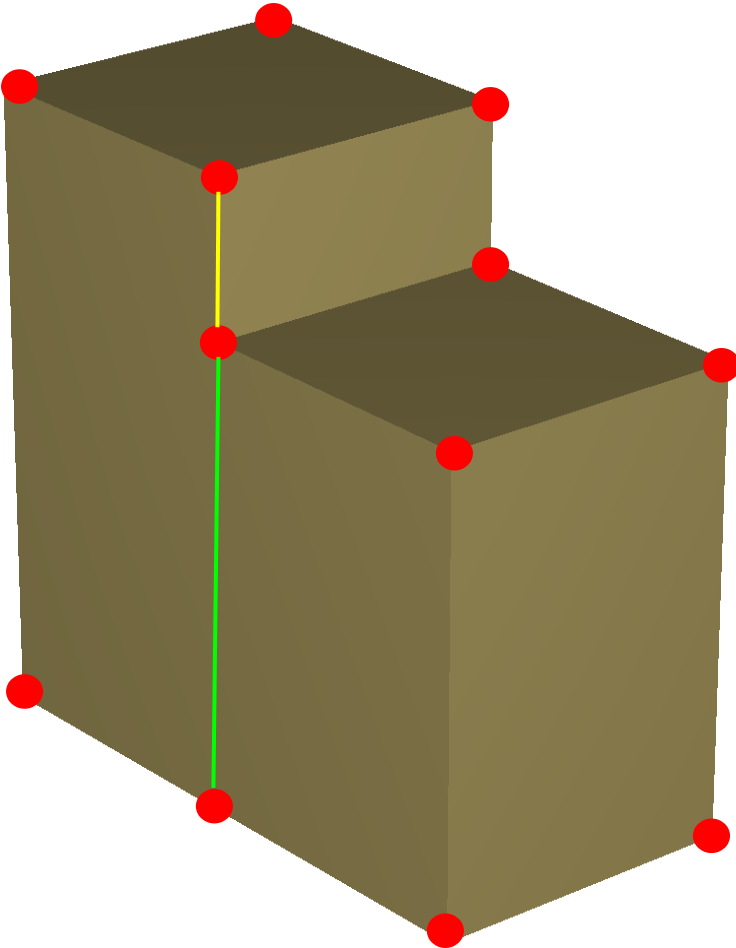
\includegraphics[width=\textwidth]{images/TetraMesh_SolidShell_EdgeExample.png}
\end{center}
\end{minipage}
\caption[Example of segment edges and corner points]
{\label{figure:SegmentEdgesAndCornerPoints} The corner points that define the bounds of two neighboring segments. The points are visualized in red, and outline the edges of the segment, describing its position in space completely. The yellow line is a vertical edge that is a short enough to be candidate for collapsing, while the green line is not. }
\end{figure*}

The top elevation of the segment is assumed to be the average of the its four top points, and the segments bottom elevation likewise the average of its four bottom points. These points do not necessarily all share the same elevation, as discussed in section \ref{section:ErosionSimulationSmoothingTheTerrainSurface}.



\subsection{Smoothing the Terrain Surface}
\label{section:ErosionSimulationSmoothingTheTerrainSurface}

The SHF alone does not accurately depict a terrain surface, because it creates a stair-case effect, as seen in Figure \ref{figure:SHFDrawn}. To smooth the surface of the terrain, segments undergo an edge collapse procedure. Vertical edges deemed short enough (such as those that represent the difference between neighbors in a layer) are collapsed, and the two points involved are replaced by a single point directly in the middle. This procedure is found in algorithm \ref{algorithm:SegmentEdgeCollapse}, and results in a smoother surface. To avoid pinching and guarantee that the algorithm converges, if two points in question belong to the same segment, their edge is not collapsed. Figure \ref{figure:SegmentEdgesAndCornerPoints} describes the difference between a collapsible edge (visualized in yellow) and a non-collapsible edge (visualized in green).

% FOR THE IMAGE, ADD A GREEN EDGE IN THE FRONT TO SHOW THAT EDGES PART OF A SEGMENT ARE NON-COLLAPSEABLE

\begin{algorithm}[t]
\begin{algorithmic}
  \STATE $numEdgesCollapsed \gets 1$
  \WHILE{$numEdgesCollapsed > 0$}
    \STATE $numEdgesCollapsed \gets 0$
    \STATE $edges = findAllEdges()$
    \FORALL{$e \in edges$}
      \IF{$e.length() < edgeThresh$}
	\STATE $collapseEdge( e )$
	\STATE $numEdgesCollapsed \gets numEdgesCollapsed + 1$
      \ENDIF
    \ENDFOR
  \ENDWHILE
\end{algorithmic}
\caption[Algorithm for segment edge collapsing]{\label{algorithm:SegmentEdgeCollapse} The procedure to collapse the edges of the SHF. The $findAllEdges()$ subroutine returns a list of vertical edges between two points that are located at the same (x, y) grid location, and have no other points between them. $numEdgesCollapsed$ is a counter that keeps track of the total number of edge collapses that occur during the algorithm, reset with every iteration. The algorithm continues to run until one pass through all edges results in no collapses, and $numEdgesCollapsed$ converges to 0.}
\end{algorithm}

Although this procedure can be performed on the SHF, it is often better to convert to a tetrahedral mesh first, as there are well documented procedures for edge collapsing on a mesh.
% , leading to fewer complications.



\subsection{Tetrahedralizing the Segmented Height Field}

For rendering and simulation particle initialization, it is necessary to convert the SHF to a tetrahedral mesh. This mesh should be closed and watertight, which means that all adjacent faces should share vertices. This is nontrivial, because neighboring segments in the SHF share no neighbor information (beyond the fact that they are in neighboring columns in a grid), and are not guaranteed to line up with one another vertically or share vertices. The following algorithm is applied to each layer individually in the SHF.

The procedure begins by tetrahedralizing every segment in the SHF. To the center of each segment, another point, which all tetrahedra share as a vertex, is added. The procedure for tetrahedralizing a single segment is shown in Figure \ref{figure:TetrahedralizeASegment}. The first step of the procedure is to divide each of the 6 segment faces in half with a diagonal edge. The second step is to connect each corner point with the center point. This results in 12 tetrahedra. Note the direction of each face's diagonal split, as this orientation is maintained throughout the entire data structure.

\begin{figure*}[t]
\centering
\begin{minipage}[b]{0.9\linewidth}
\begin{center}
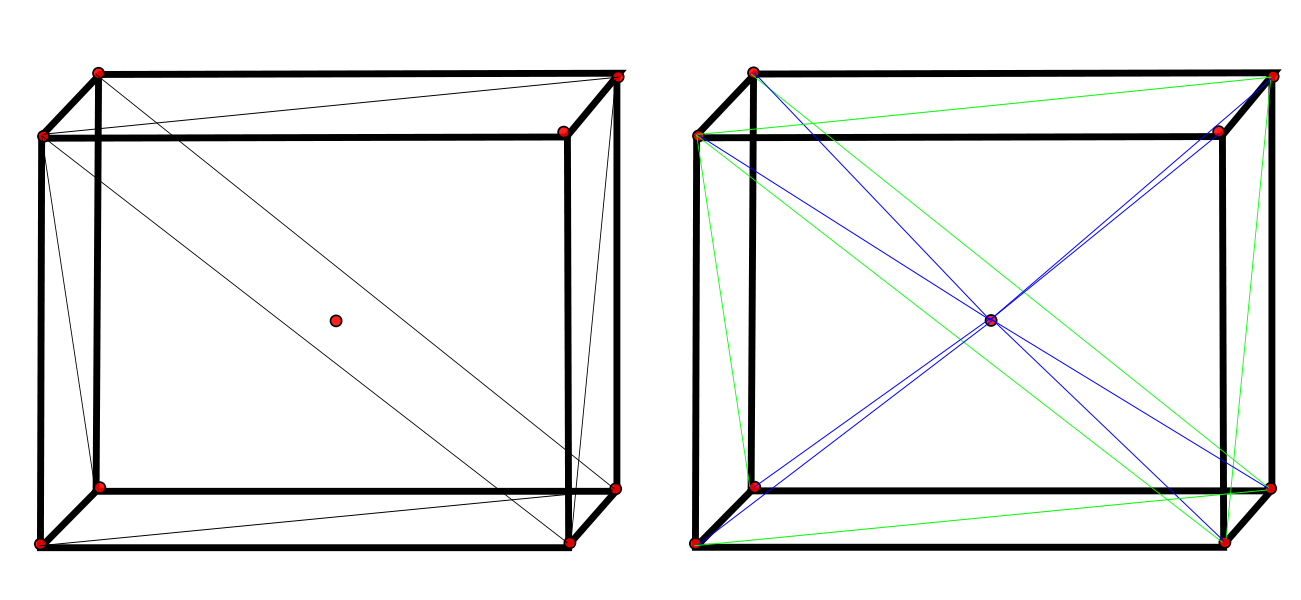
\includegraphics[width=\textwidth]{images/DividingASegment.png}
\end{center}
\end{minipage}
\caption[Tetrahedralizing a segment]
{\label{figure:TetrahedralizeASegment} The procedure for tetrahedralizing a single segment. The first step, shown in the left image, splits each face of the segment with a diagonal edge. Each of the segments corner points are then connected to the center point, creating 12 distinct adjacent tetrahedra. }
\end{figure*}

While the original segment tetrahedralizing creates a mesh, it is not watertight (there are NULL faces, or adjacent faces that are abutting but share only two of three vertices). This must be rectified in order to achieve a watertight mesh. Solving this problem is a three step process, one for each of the issues that arise. Figure \ref{figure:TwoStepTetraProcess} presents two such issues. Situations A) and B) arise from abutting tetrahedral faces with edges that do not share points. The first step is to make sure that no tetrahedral edge contains a point that is not an end point. In situation A), there are two red points located on the edges of the abutting tetrahedra. The solution to this is to subdivide the tetrahedra whose edges are disrupted into two tetrahedra, as seen as the solution on line A).

Once all edges that must be subdivided are, another problem arises. The larger segment in row B) contains a tetrahedron whose edge bisects the edge of a tetrahedra of its neighbor. This problem is solved by performing a tetrahedra diagonal swapping algorithm, during which each pair of tetrahedra who have faces that share a normal vector (such as the two blue ones in question) are checked to see if their diagonals should be swapped. If the new diagonal would be shorter than the current one, then a swap takes place. This process guarantees that every pair of abutting tetrahedra that share vertices are split with the same (shortest) diagonal, thus making the mesh watertight. This procedure is described by algorithm \ref{algorithm:TetraSwapping}, and by row B) in Figure \ref{figure:TwoStepTetraProcess}.

\begin{figure}[t]
\begin{minipage}{0.9\linewidth}
\centering
\begin{minipage}{0.48\textwidth}
\begin{center}
\textbf{Problem}
\end{center}
\end{minipage}
\begin{minipage}{0.48\textwidth}
\begin{center}
\textbf{Solution}
\end{center}
\end{minipage}
\\
A
\begin{minipage}{0.25\textwidth}
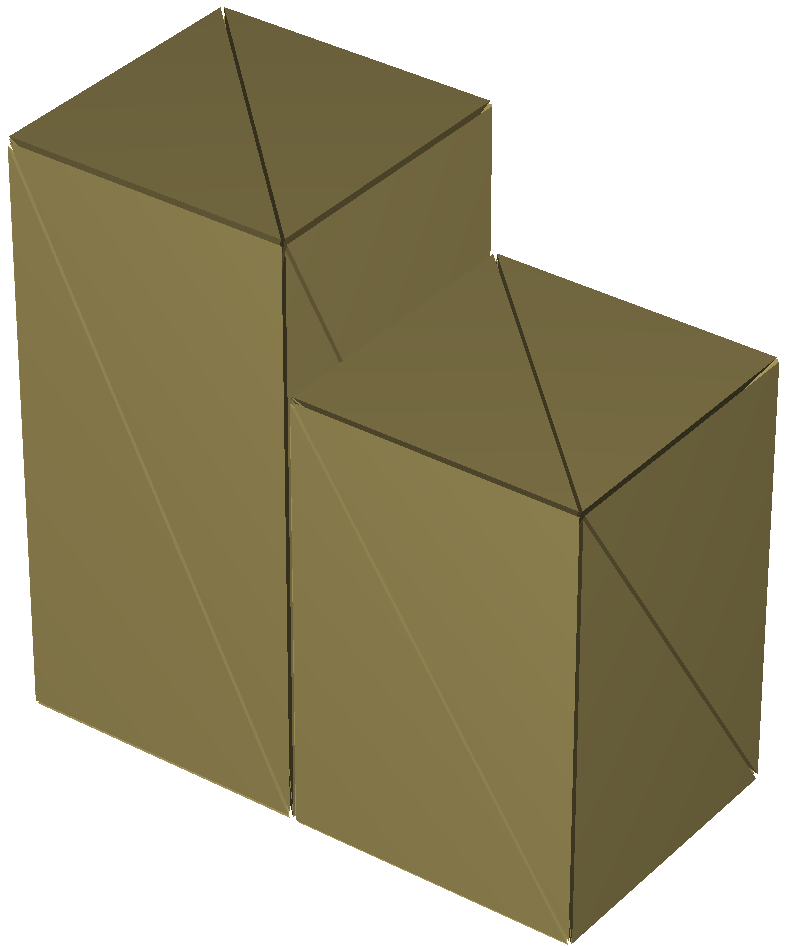
\includegraphics[width=\textwidth]{images/TetraMesh_WithNullFaces_crop.png}
\end{minipage}
\begin{minipage}{0.45\textwidth}
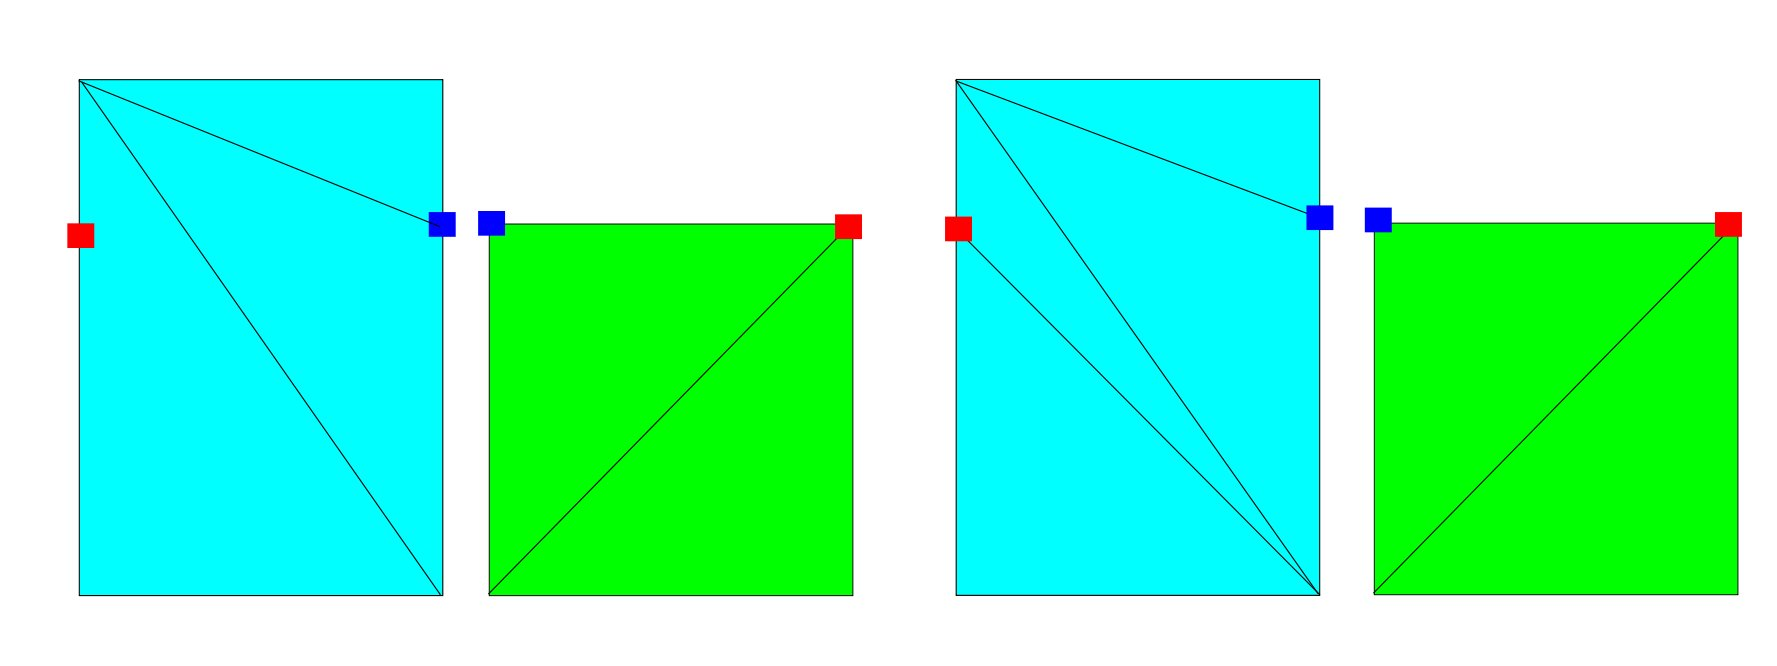
\includegraphics[width=\textwidth]{images/Subdivision_Example_2.jpg}
\end{minipage}
\begin{minipage}{0.25\textwidth}
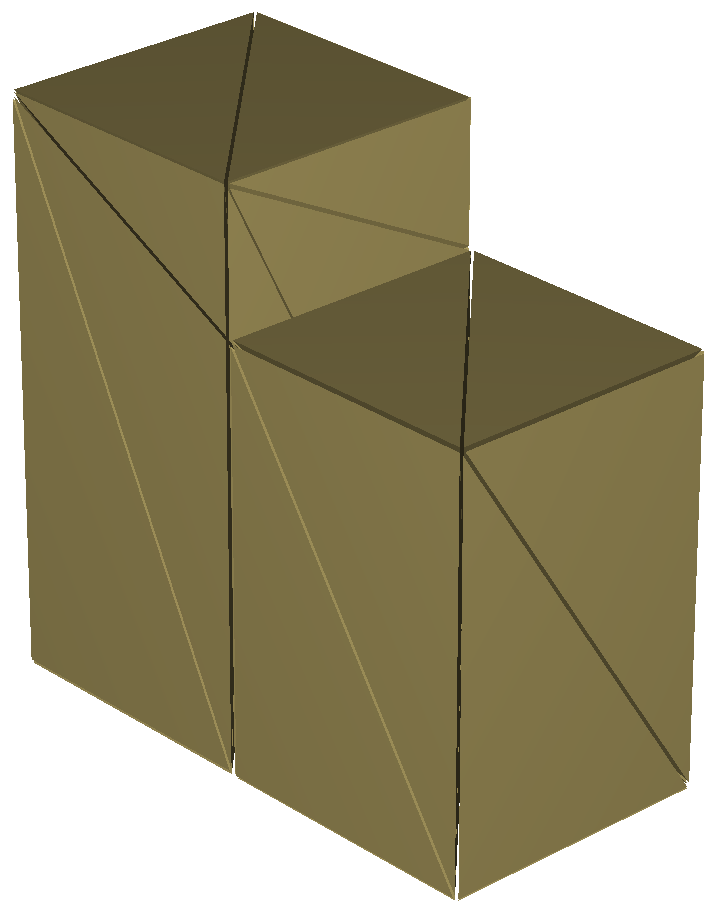
\includegraphics[width=\textwidth]{images/TetraMesh_WithNullFaces_AfterSubdivision_crop.png}
\end{minipage}
\\
B
% \begin{minipage}{0.65\textwidth}
% 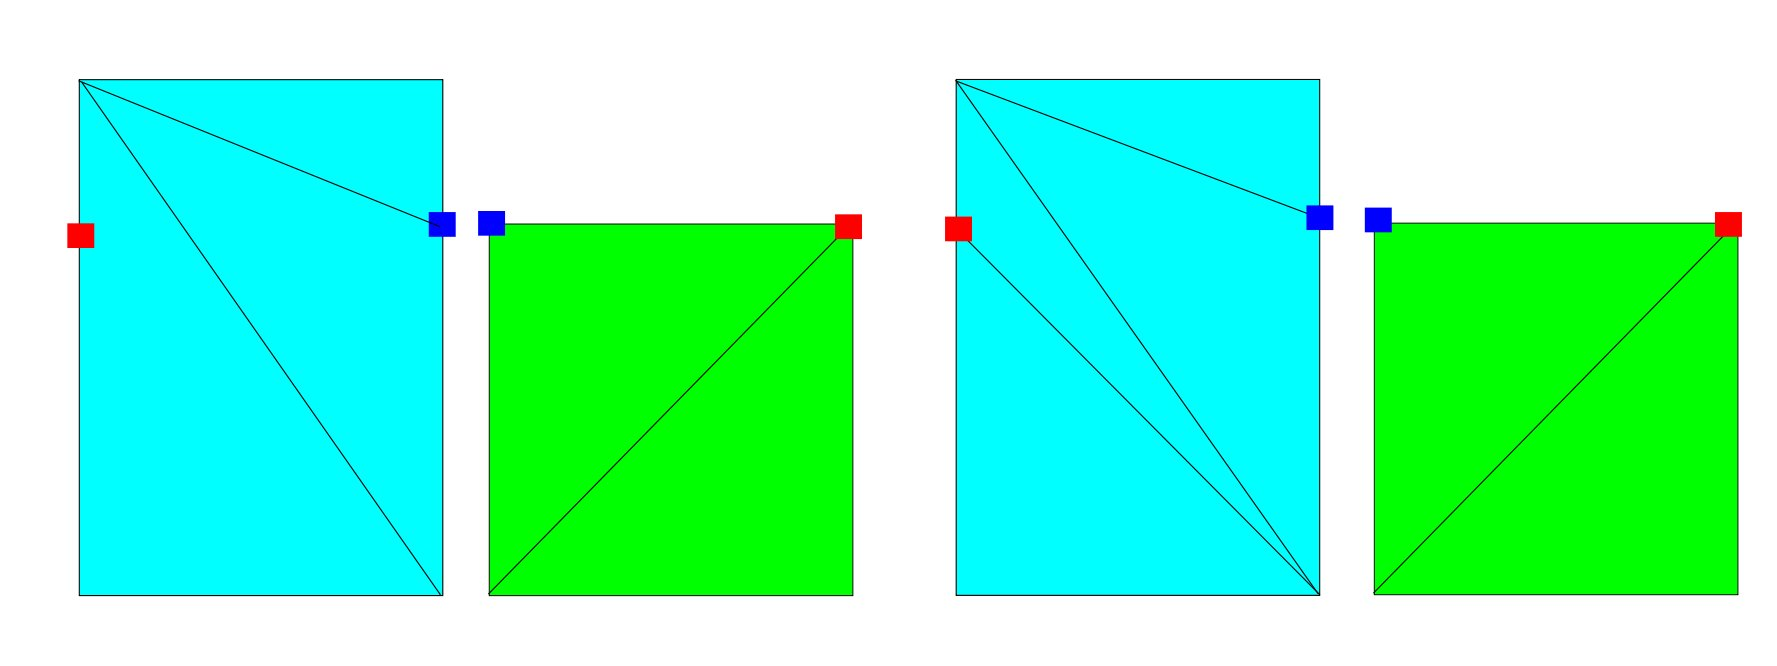
\includegraphics[width=\textwidth]{images/Subdivision_Example_2.jpg}
% \end{minipage}
% \begin{minipage}{0.3\textwidth}
% 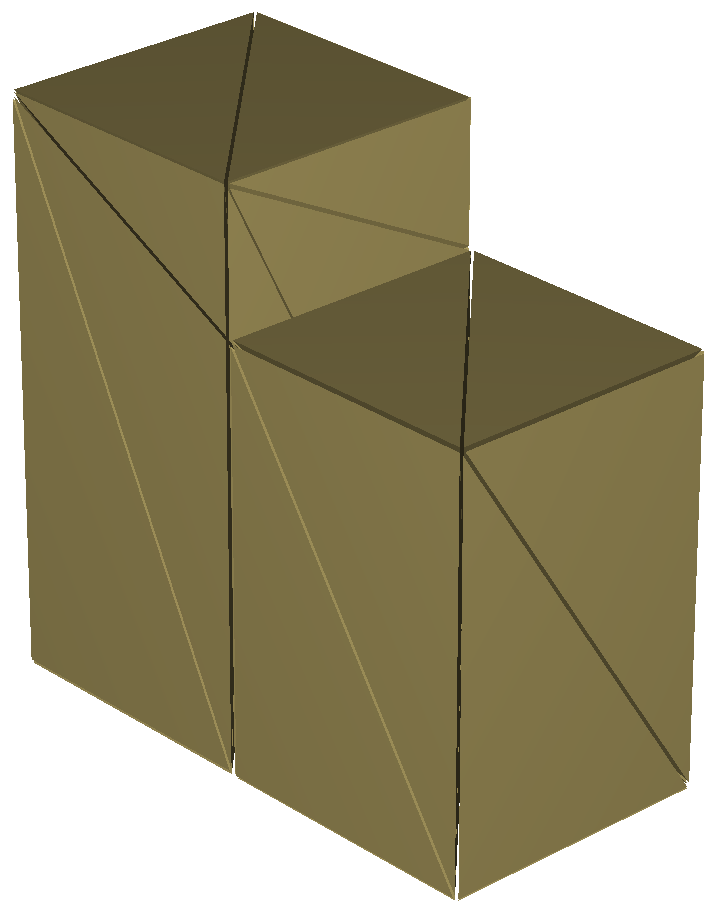
\includegraphics[width=\textwidth]{images/TetraMesh_WithNullFaces_AfterSubdivision_crop.png}
% \end{minipage}
% \\
% C
\begin{minipage}{0.25\textwidth}
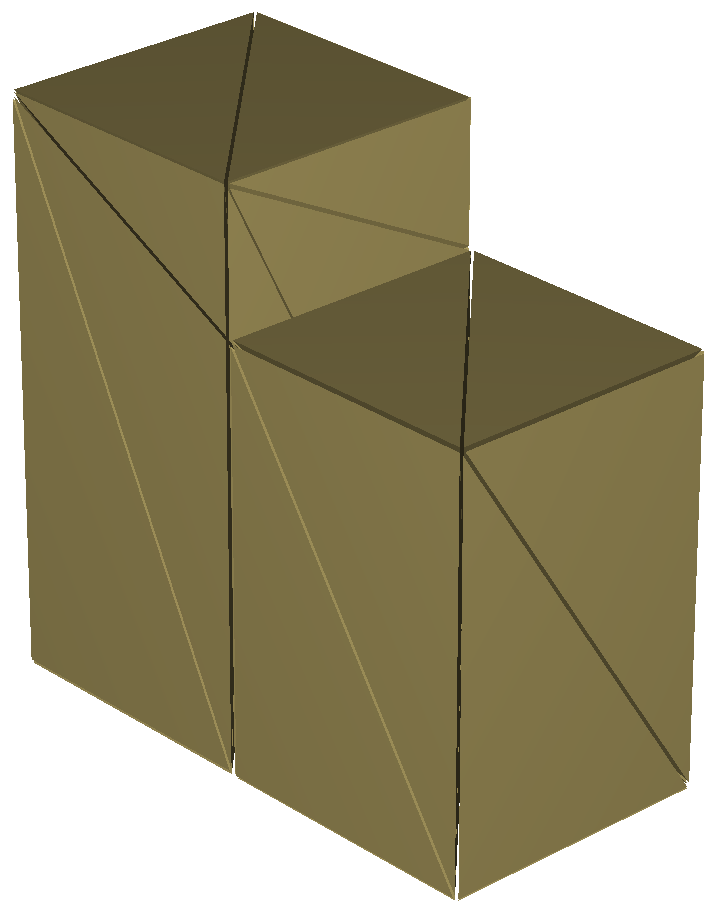
\includegraphics[width=\textwidth]{images/TetraMesh_WithNullFaces_AfterSubdivision_crop.png}
\end{minipage}
\begin{minipage}{0.45\textwidth}
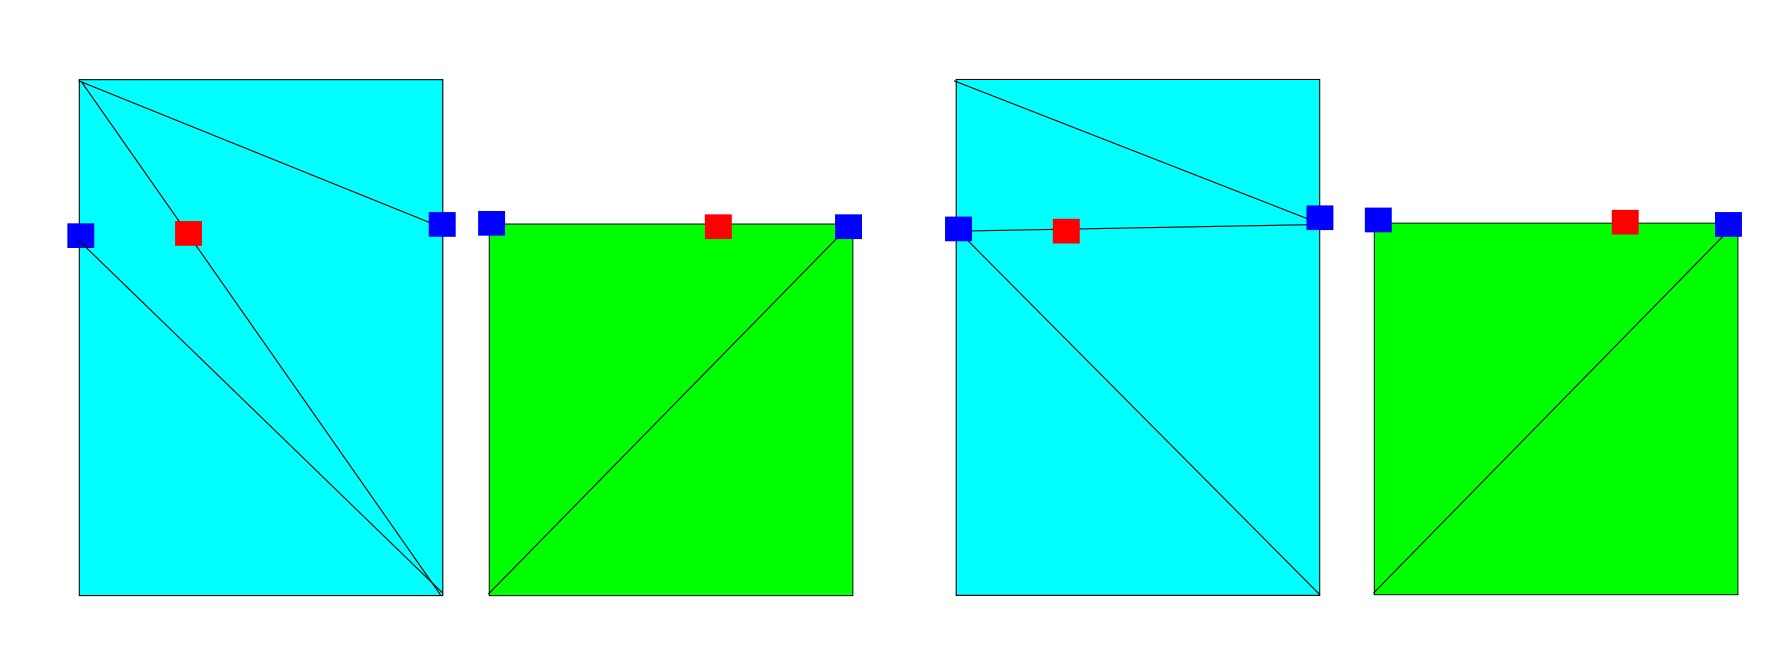
\includegraphics[width=\textwidth]{images/Subdivision_Example_3.jpg}
\end{minipage}
\begin{minipage}{0.25\textwidth}
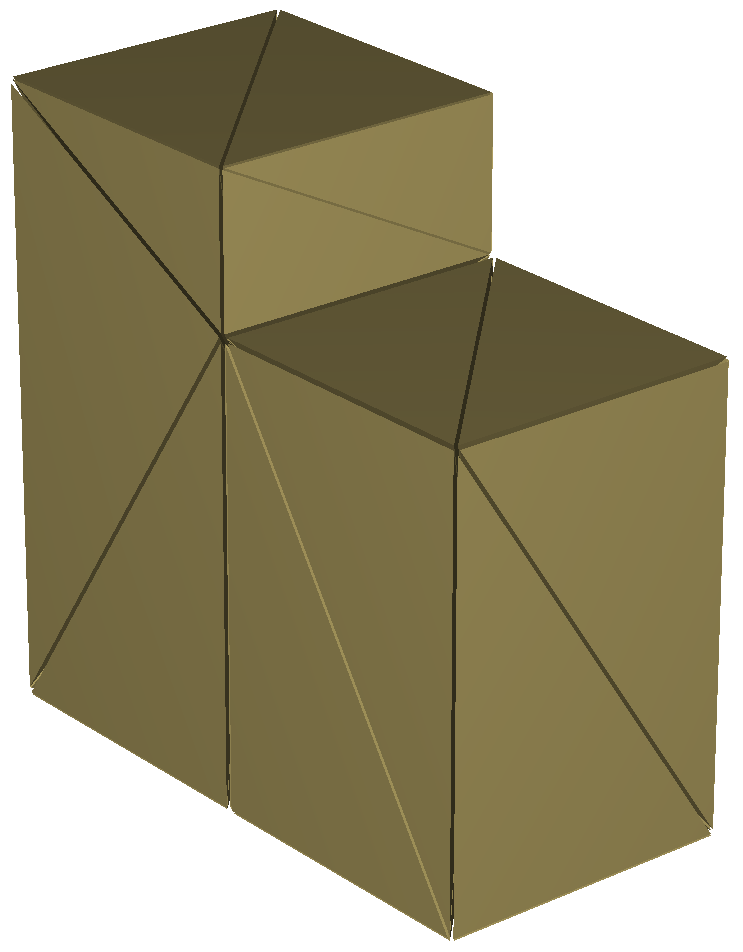
\includegraphics[width=\textwidth]{images/TetraMesh_AfterSubdivision_AndSwapping_crop.png}
\end{minipage}
\\
\end{minipage}
\caption[Two-step process for creating a watertight tetrahedral mesh from a SHF with tetrahedralized segments]
{\label{figure:TwoStepTetraProcess} The two-step process for creating a watertight tetrahedral mesh from a SHF with tetrahedralized segments. Each row is a pipeline, moving from the problem on the left to the solution and and result on the right. Red points represent corresponding problem points, while dark blue points represent the solutions. The two problems that are presented are A) two NULL faces are abutting and their edges need to be subdivided, and B) the subdivided tetrahedra have an edge that cross an edge of an abutting tetrahedron. Problem A) is solved by subdividing edges by inserting new points, and B) is solved by swapping diagonals of neighboring tetrahedra that share an edge.}
\end{figure}

% THIS FIGURE ^ NEEDS TO BE FIXED!!!

\begin{algorithm}[t]
\begin{algorithmic}
  \FORALL{$t \in allTetrahedra()$}
    \FORALL{$n \in neighborsOfT()$}
      \FORALL{$f \in facesOfTetra( t )$}
	\FORALL{$f2 \in facesOfTetra( n )$}
	  \IF{ $sameNormal( f, f2 )$ }
	    \STATE $curLength \gets lengthOfCurrentDiagonal( f, f2 )$
	    \STATE $possibleLength \gets lengthOfPossibleDiagonal( f, f2 )$
	    \IF{ $possibleLength < curLength$ }
	      \STATE $swapDiagonals( f, f2 )$
	    \ENDIF
	  \ENDIF
	\ENDFOR
      \ENDFOR
    \ENDFOR
  \ENDFOR
\end{algorithmic}
\caption[Algorithm for tetra swapping]
{\label{algorithm:TetraSwapping} The procedure to swap the diagonals of neighboring tetrahedra whose faces share a normal vector. Find the faces that share a normal vector (face in the same direction), and compare the lengths of pre- and post-swap diagonals. If swapping creates a shorter diagonal, perform the swap. The algorithm relies on the fact that, if faces from neighboring tetrahedra share a normal vector, then the pair is unique.}
\end{algorithm}

This watertight tetrahedral mesh can be exported to a ray tracer or modeling program, and can also have the edge collapsing algorithm presented in section \ref{section:ErosionSimulationSmoothingTheTerrainSurface} performed on it. An example of a ray-traced tetrahedral mesh from the simulation is seen in Figure \ref{figure:RayTracedTetrahedralMesh}.

\begin{figure*}[t]
\centering
\begin{minipage}[b]{0.9\linewidth}
\begin{center}
\includegraphics[width=\textwidth]{images/SegmentedHeightField_RayTracedExample_crop.png}
\end{center}
\end{minipage}
\caption[Ray-traced example of tetrahedral mesh from the erosion simulation]
{\label{figure:RayTracedTetrahedralMesh} A ray-traced example of the tetrahedral mesh from a time step in the middle of an erosion simulation.
% Note that this example has not been edge-collapsed. 
}
\end{figure*}




\section{The Smoothed Particle Hydrodynamics Simulation}

% \fbox{Add some images here of SPH stuff}

In addition to the soil model, the erosion simulation requires a fluid model, the Smoothed Particle Hydrodynamics simulation. SPH models the water as a series of particles, each of which maintains its own mass and velocity. The behavior of the particles is modeled by the Navier-Stokes equation for conservation of momentum, used to update the velocity and position of the particles each time step of the simulation:

\begin{equation}
  \rho\left(\dfrac{\delta v}{\delta t} + v \nabla v \right) = - \nabla p + \rho g + \mu \nabla^{2} v
\end{equation}

\noindent where $\rho$ is the fluid density, $v$ is velocity, $p$ is pressure, $g$ is the external force field, and $\mu$ is the dynamic viscosity. Normally, special attention must be paid to conservation of mass, but the SPH system guarantees that mass is maintained, and so this can be ignored.
% portion of the system is omitted.

The resolution of the system is dependent upon the particle spacing, one of the parameters to the system. A smaller initial spacing means more particles and therefore a more accurate simulation. However, more particles means more resources are required to calculate the simulation time steps, thus limiting the simulation's attainable accuracy. A particle spacing of 0.004 m was used for the trials of the simulation.
% , generates approximately 450,000 particles. 

Another parameter to the system is the smoothing length, a radius of influence for each particle. Particles within a smoothing length distance of one another influence each other during the Navier-Stokes calculation. Trials have shown that the smoothing length set to double the particle spacing assures an adequate number of particles fall within the area of influence.

The third and final parameter to the system is the length of a single time step. If it is too long, then the simulation will sacrifice accuracy by allowing the particles to travel too far each time step. If the time step is too short, computation time increases. Balancing these situations, a time step of 0.001 seconds was selected for the trials. 
The values for each of these parameters are independent of simulation geometry, so they remain the same regardless of situation.

The simulation also requires the placement of a source and a sink. These greatly influence the flow of water, and are geometry dependent. For instance, when simulation water flows over a levee, the source should be on the wet side of the levee and the sink on the dry. The source is responsible for setting an initial flow rate of the water, which dictates the velocities of the particles as they appear in the system. In addition, the rate at which particles are generated is situation dependent. Flow rate and source and sink placement are simulation specific parameters.


\section{The Erosion Simulation}

The erosion simulation couples the SHF levee model with the SPH fluid model by converting the SHF into a series of soil particles, arranged in a lattice pattern. Unlike the water particles, the soil particles have no velocity, instead storing a material type (and, by extension, storing all material properties of the soil), and a percentage of volume. Generally, the resolution of the soil particles are higher than that of the water particles, approximately 0.003m between point samples. 

Soil particles have a smaller spacing in part because the surface particles must act as a boundary for the fluid simulation. To accomplish this, the system includes a repellent force between soil and water particles, as proposed by Amada \cite{amada-particles}:

\begin{equation}
  \vec{f} = \left( K_{S} d - \left( \vec{v} \cdot \vec{n} \right) K_{D} \right) \vec{n}
\end{equation}

\noindent where $K_{S}$ is the penalty force stiffness, $K_{D}$ is the damping coefficient for the velocity
$\vec{v}$ of an approaching fluid particle, $d$ is the penetrated distance measured normal to the
boundary, and $\vec{n}$ is the surface normal. 
This force dampens the velocity of any incoming water particles, increasing acceleration away from the boundary. 

Erosion is simulated using the model presented by Briaud \cite{Briaud-ErosionByOvertopping}. Water particles that flow over the soil boundary exert a shear stress on the soil particles. One of the material properties in the system is the \emph{soil erodibility}, as discussed in Section \ref{section:SoilErodibility}, that provides a relationship between the shear stress on the soil and its rate of erosion. The system calculates the rate of erosion by the equation:

\begin{equation}
\label{equation:ShearStress}
  z\left(\mu\right) = \alpha \mu + c
\end{equation}

\noindent where $\mu$ is the shear stress, $\alpha$ is the erodibility, and $c$ is the ``critical shear stress'', a threshold for shear stress under which no erosion occurs.

The rate of erosion dictates the rate at which volume is lost by the soil particle. Once the soil particle's volume reaches 0\%, it is removed from the system. As part of the system's optimization, only the soil particles that can interact with water at any given point in time are considered ``active'', and are placed in a boundary particle list. When one is removed, the system replaces it with any new particles on the boundary.

\section{Simulation Experiment and Results}
\label{section:ErosionSimulationResults}

Two separate experiments were performed. The first provided visual validation of the simulation by comparison to the laboratory experiments described 
by Kalamzare et al. \cite{Kamalzare-ValidationOfErosionModeling} and Gross et al. \cite{gross_icse_2010}.
% in Section \ref{section:LaboratoryExperimentation}. 
The second set of experiments tested various system parameters, including water flow rate, levee geometry, and soil erodibility.

\subsection{Visual Comparison to Laboratory Experiments}

\begin{figure}[t]
	\centering 
	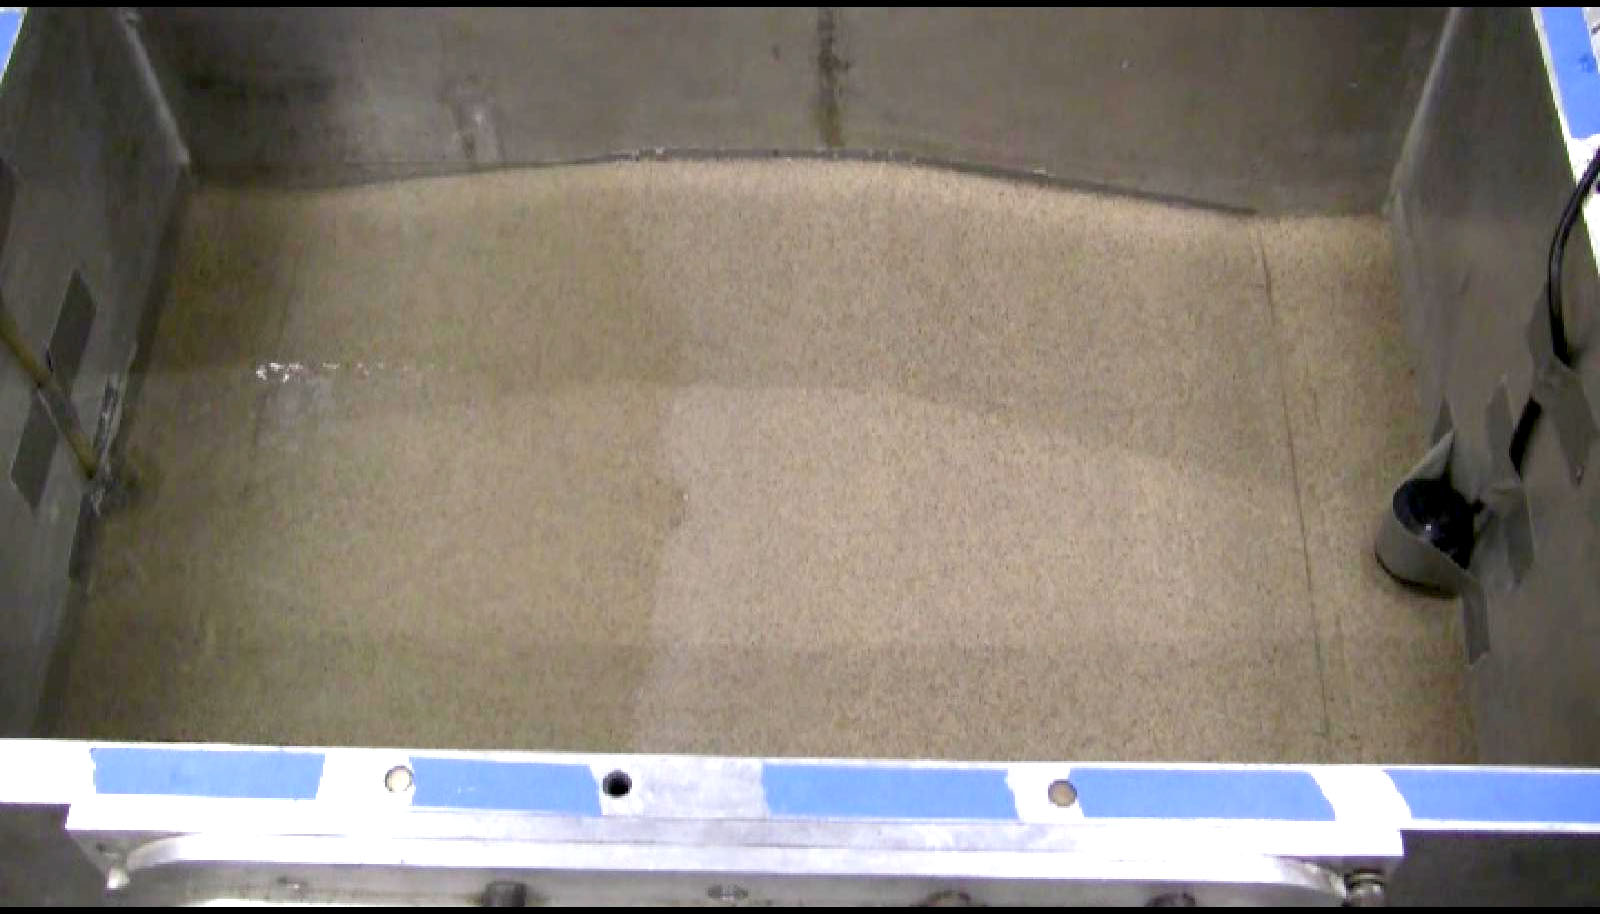
\includegraphics[width=0.32\linewidth]{images/InitialOvertopping_flip.jpg}
	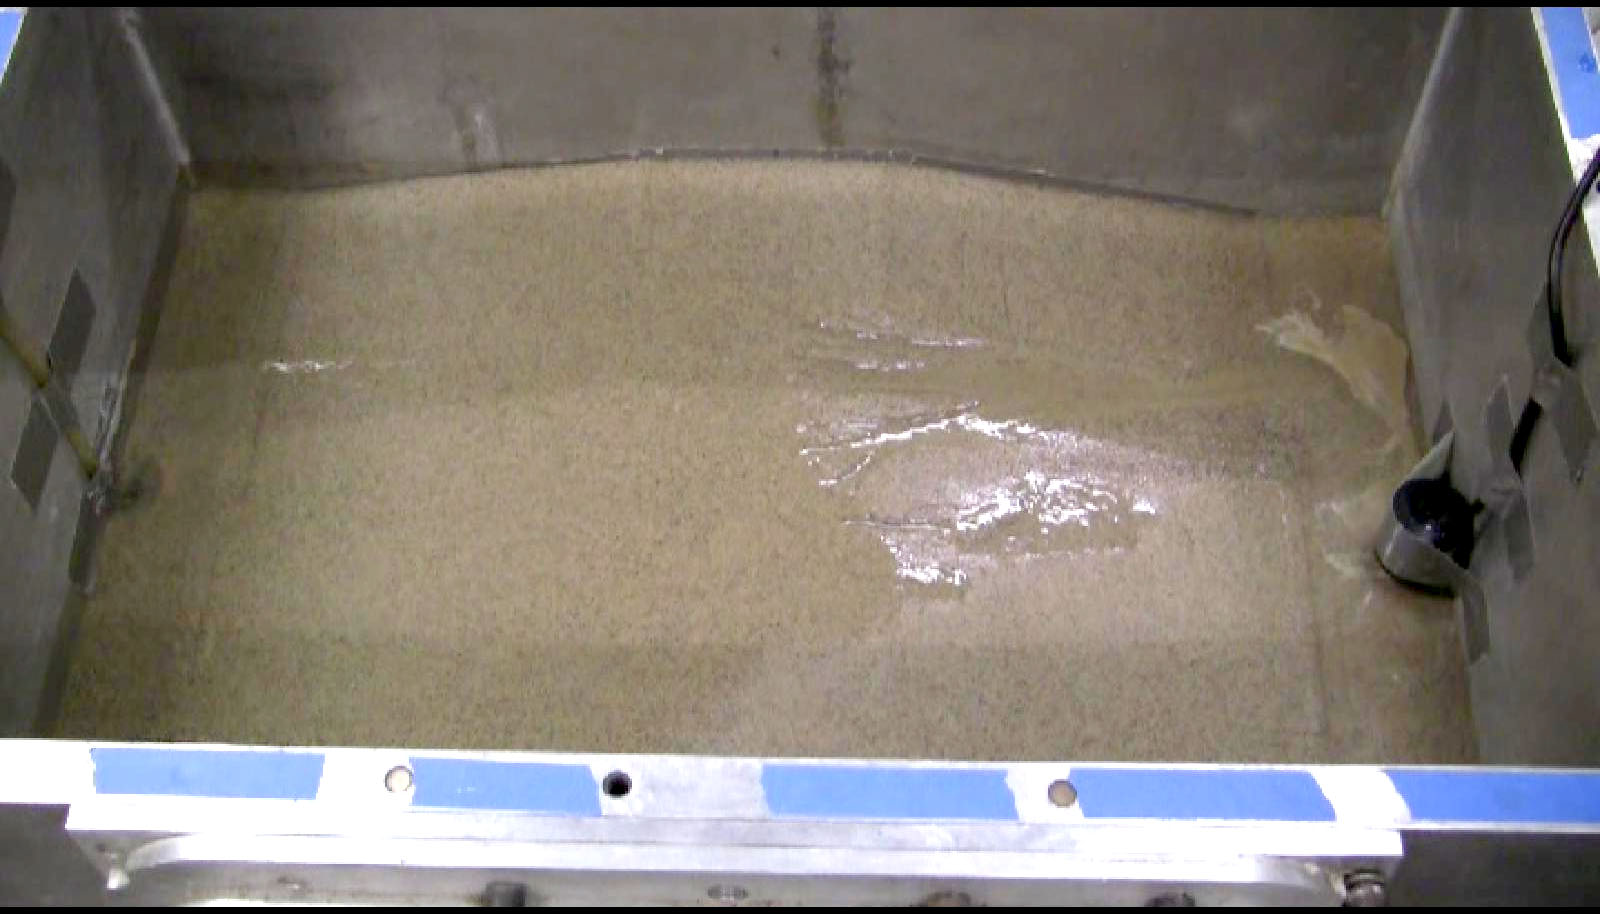
\includegraphics[width=0.32\linewidth]{images/ChannelsForm_flip.jpg}
	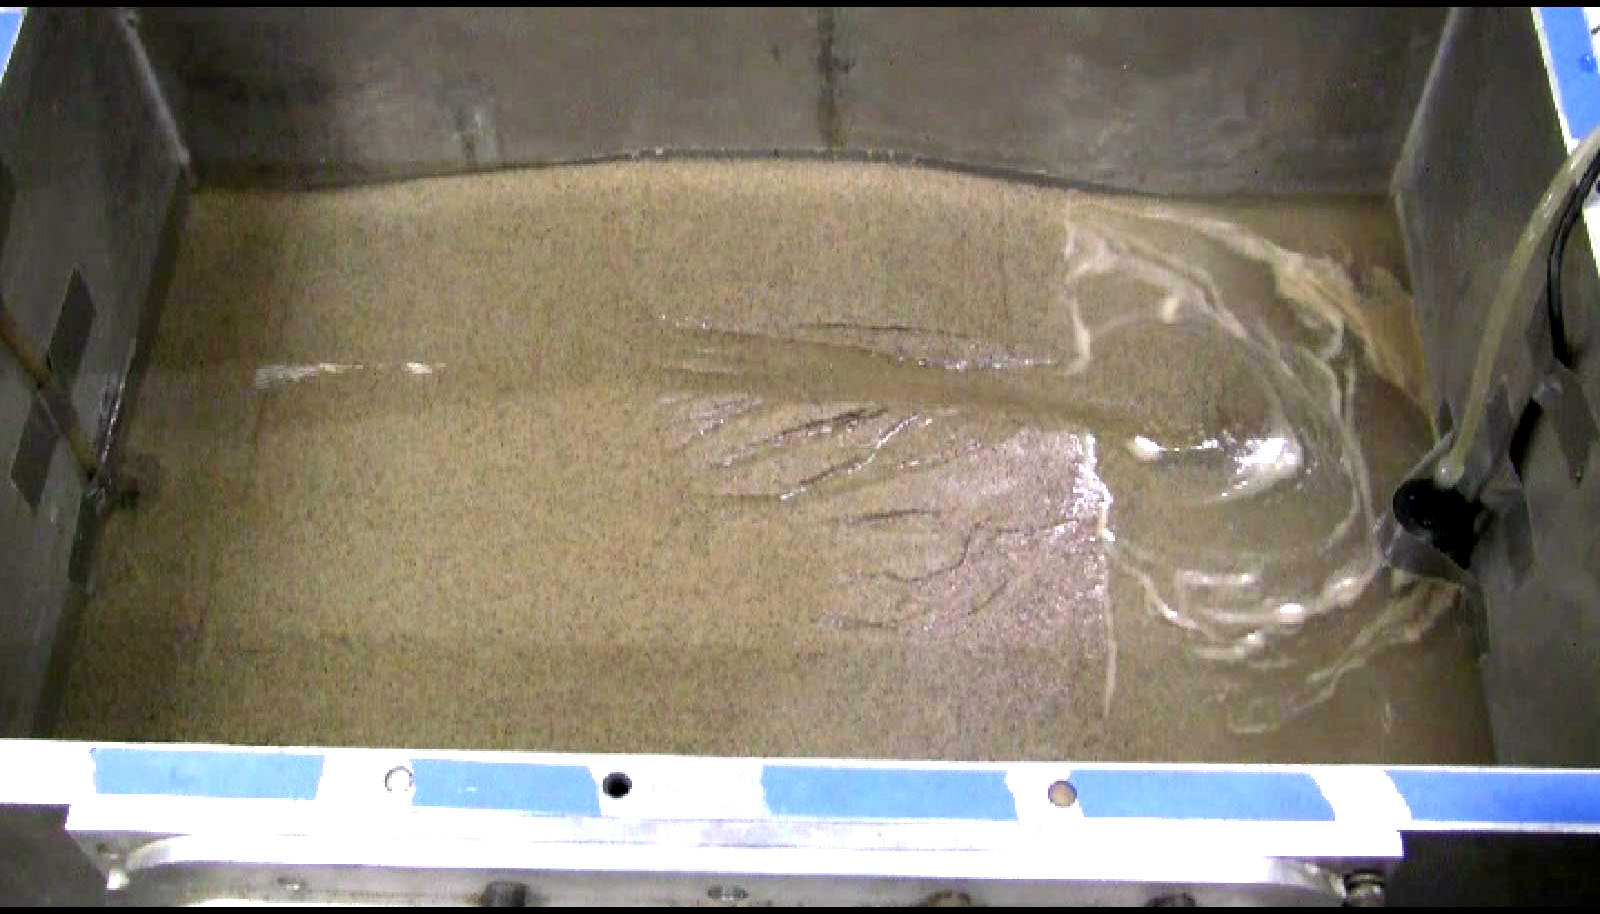
\includegraphics[width=0.32\linewidth]{images/BreachFormation_flip.jpg}
\caption[Images from laboratory experiment]{\label{figure:physical_experiment}Images from a video of a
  physical experiment using pure sand.  From left to right these
  images capture the moment that water begins to overtop the crest of
  the levee, the formation of rills on the downslope of the levee, and
  the moment of breach of the levee, when a channel has cut through
  the full width of the crest of the levee.}
\end{figure}

\begin{figure}
\begin{minipage}{0.98\textwidth}
			\centering
			\begin{tabular}{@{}r@{~}|@{~}c@{~}|@{~}c@{~}|@{~}c@{~}|@{~}c@{~}|@{~}c@{~}|@{~}c@{~}|@{~}c@{~}|@{~}c@{~}|@{~}c@{~}|@{~}c@{~}|}
				\multicolumn{2}{c}{~~~~~sand-clay}&
				\multicolumn{1}{c}{}&
				\multicolumn{1}{c}{}&
				\multicolumn{1}{c}{}&
				\multicolumn{1}{c}{pure sand}
				\\ 

% 				\begin{sideways}Min.\end{sideways}

				&
				\#1&%\#2 & 
				\#2&%\#4 & 
				\#3&%\#6 & 
				\#4&%\#8 & 
				%\#9&
				\#5 
		% 		\\ 
		% 		& 
		% 		$a=93$ & $a=93$ &
		% 		$a=115$ & $a=115$ &
		% 		$a=137$ & $a=137$ &
		% 		$a=159$ & $a=159$ &
		% 		$a=187$ & $a=187$ 
		% 		\\ 
		% 		&
		% 		$\tau_c=3.00$ & $\tau_c=2.00$ & 
		% 		$\tau_c=2.75$ & $\tau_c=2.75$ & 
		% 		$\tau_c=2.50$ & $\tau_c=2.50$ & 
		% 		$\tau_c=2.25$ & $\tau_c=2.25$ & 
		% 		$\tau_c=3.00$ & $\tau_c=2.00$ 
				\\ \hline

				\begin{sideways}\begin{small}~~1 min~~~\end{small}\end{sideways}& 
				\resizebox{0.13\textwidth}{0.43in}{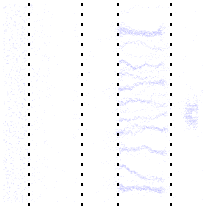
\includegraphics{simulation_images/93_2/93_2_01mins_d.png}}&
				% \resizebox{0.13\textwidth}{0.43in}{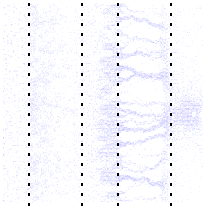
\includegraphics{simulation_images/93_1/93_1_01mins_d.png}}&
				\resizebox{0.13\textwidth}{0.43in}{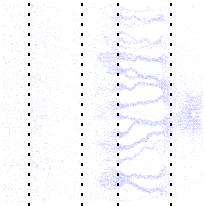
\includegraphics{simulation_images/115_1/115_1_01mins_d.png}}& 
				% \resizebox{0.13\textwidth}{0.43in}{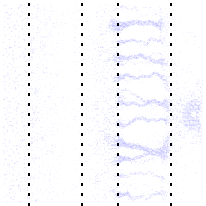
\includegraphics{simulation_images/115_2/115_2_01mins_d.png}}& 
				\resizebox{0.13\textwidth}{0.43in}{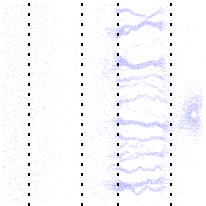
\includegraphics{simulation_images/137_1/137_1_01mins_d.png}}& 
				% \resizebox{0.13\textwidth}{0.43in}{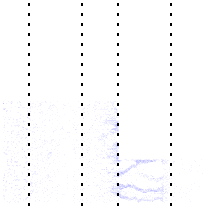
\includegraphics{simulation_images/137_2/137_2_01mins_d.png}}& 
				\resizebox{0.13\textwidth}{0.43in}{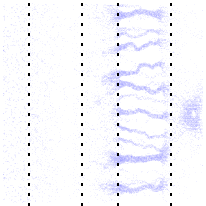
\includegraphics{simulation_images/159_1/159_1_01mins_d.png}}& 
				% \resizebox{0.13\textwidth}{0.43in}{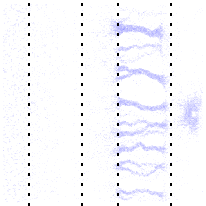
\includegraphics{simulation_images/159_2/159_2_01mins_d.png}}& 
% 				\resizebox{0.13\textwidth}{0.43in}{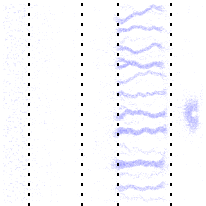
\includegraphics{simulation_images/187_1/187_1_01mins_d.png}}
				\resizebox{0.13\textwidth}{0.43in}{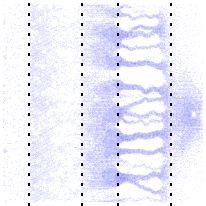
\includegraphics{simulation_images/187_2/187_2_01mins_d.png}}  
				\\ \hline 
				%
				\begin{sideways}\begin{small}~~2 min~~~\end{small}\end{sideways}& 
				\resizebox{0.5in}{0.43in}{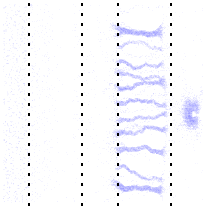
\includegraphics{simulation_images/93_2/93_2_02mins_d.png}}&
				% \resizebox{0.13\textwidth}{0.43in}{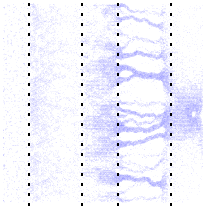
\includegraphics{simulation_images/93_1/93_1_02mins_d.png}}&
				\resizebox{0.5in}{0.43in}{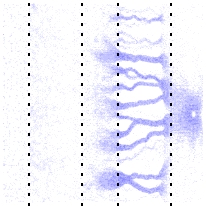
\includegraphics{simulation_images/115_1/115_1_02mins_d.png}}& 
				% \resizebox{0.13\textwidth}{0.43in}{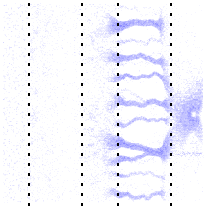
\includegraphics{simulation_images/115_2/115_2_02mins_d.png}}& 
				\resizebox{0.5in}{0.43in}{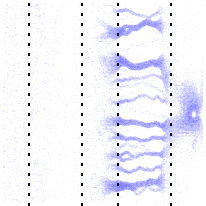
\includegraphics{simulation_images/137_1/137_1_02mins_d.png}}& 
				% \resizebox{0.13\textwidth}{0.43in}{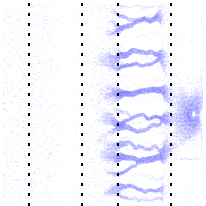
\includegraphics{simulation_images/137_2/137_2_02mins_d.png}}& 
				\resizebox{0.5in}{0.43in}{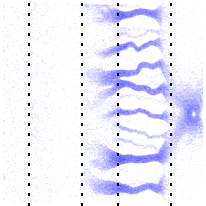
\includegraphics{simulation_images/159_1/159_1_02mins_d.png}}& 
				% \resizebox{0.13\textwidth}{0.43in}{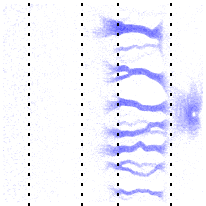
\includegraphics{simulation_images/159_2/159_2_02mins_d.png}}& 
% 				\resizebox{0.5in}{0.43in}{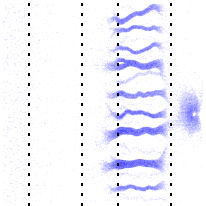
\includegraphics{simulation_images/187_1/187_1_02mins_d.png}}
				\resizebox{0.13\textwidth}{0.43in}{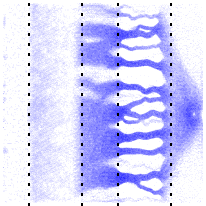
\includegraphics{simulation_images/187_2/187_2_02mins_d.png}}  
				\\ \hline 
				%
				\begin{sideways}\begin{small}~~3 min~~~\end{small}\end{sideways}& 
				\resizebox{0.13\textwidth}{0.43in}{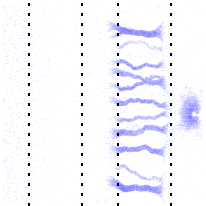
\includegraphics{simulation_images/93_2/93_2_03mins_d.png}}&
				% \resizebox{0.13\textwidth}{0.43in}{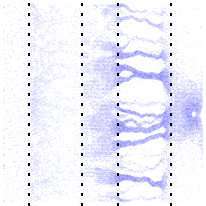
\includegraphics{simulation_images/93_1/93_1_03mins_d.png}}&
				\resizebox{0.13\textwidth}{0.43in}{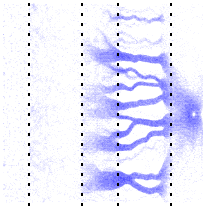
\includegraphics{simulation_images/115_1/115_1_03mins_d.png}}& 
				% \resizebox{0.13\textwidth}{0.43in}{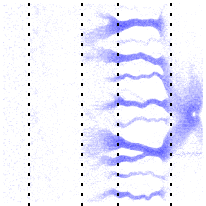
\includegraphics{simulation_images/115_2/115_2_03mins_d.png}}& 
				\resizebox{0.13\textwidth}{0.43in}{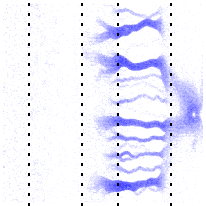
\includegraphics{simulation_images/137_1/137_1_03mins_d.png}}& 
				% \resizebox{0.13\textwidth}{0.43in}{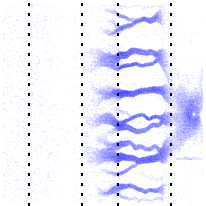
\includegraphics{simulation_images/137_2/137_2_03mins_d.png}}& 
				\resizebox{0.13\textwidth}{0.43in}{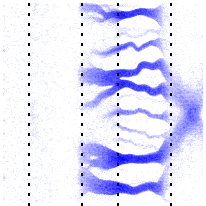
\includegraphics{simulation_images/159_1/159_1_03mins_d.png}}& 
				% \resizebox{0.13\textwidth}{0.43in}{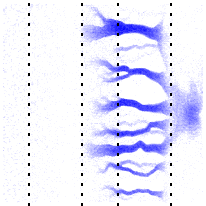
\includegraphics{simulation_images/159_2/159_2_03mins_d.png}}& 
% 				\resizebox{0.13\textwidth}{0.43in}{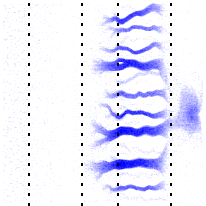
\includegraphics{simulation_images/187_1/187_1_03mins.png}}
				\resizebox{0.13\textwidth}{0.43in}{\includegraphics{simulation_images/187_2/187_2_03mins_d.png}}  
				\\ \hline 
				%
				\begin{sideways}\begin{small}~~4 min~~~\end{small}\end{sideways}& 
				\resizebox{0.5in}{0.43in}{\includegraphics{simulation_images/93_2/93_2_04mins_d.png}}&
				% \resizebox{0.13\textwidth}{0.43in}{\includegraphics{simulation_images/93_1/93_1_04mins_d.png}}&
				\resizebox{0.5in}{0.43in}{\includegraphics{simulation_images/115_1/115_1_04mins_d.png}}& 
				% \resizebox{0.13\textwidth}{0.43in}{\includegraphics{simulation_images/115_2/115_2_04mins_d.png}}& 
				\resizebox{0.5in}{0.43in}{\includegraphics{simulation_images/137_1/137_1_04mins_d.png}}& 
				%\resizebox{0.13\textwidth}{0.43in}{\includegraphics{simulation_images/137_2/137_2_04mins_d.png}}& 
				\resizebox{0.5in}{0.43in}{\includegraphics{simulation_images/159_1/159_1_04mins_d.png}}& 
				%\resizebox{0.13\textwidth}{0.43in}{\includegraphics{simulation_images/159_2/159_2_04mins_d.png}}& 
% 				\resizebox{0.5in}{0.43in}{\includegraphics{simulation_images/187_1/187_1_04mins_d.png}}
				\resizebox{0.13\textwidth}{0.43in}{\includegraphics{simulation_images/187_2/187_2_04mins_d.png}} 
				\\ \hline 
				% 
				\begin{sideways}\begin{small}~~5 min~~~\end{small}\end{sideways}& 
				\resizebox{0.13\textwidth}{0.43in}{\includegraphics{simulation_images/93_2/93_2_05mins_d.png}}&
				%\resizebox{0.13\textwidth}{0.43in}{\includegraphics{simulation_images/93_1/93_1_05mins_d.png}}&
				\resizebox{0.13\textwidth}{0.43in}{\includegraphics{simulation_images/115_1/115_1_05mins_d.png}}& 
				%\resizebox{0.13\textwidth}{0.43in}{\includegraphics{simulation_images/115_2/115_2_05mins_d.png}}& 
				\resizebox{0.13\textwidth}{0.43in}{\includegraphics{simulation_images/137_1/137_1_05mins_d.png}}& 
				%\resizebox{0.13\textwidth}{0.43in}{\includegraphics{simulation_images/137_2/137_2_05mins_d.png}}& 
				\resizebox{0.13\textwidth}{0.43in}{\includegraphics{simulation_images/159_1/159_1_05mins_d.png}}& 
				%\resizebox{0.13\textwidth}{0.43in}{\includegraphics{simulation_images/159_2/159_2_05mins_d.png}}& 
% 				\resizebox{0.13\textwidth}{0.43in}{\includegraphics{simulation_images/187_1/187_1_05mins_d.png}}
				\resizebox{0.13\textwidth}{0.43in}{\includegraphics{simulation_images/187_2/187_2_05mins_d.png}}  
				\\ \hline 
				% 
				\begin{sideways}\begin{small}~~6 min~~~\end{small}\end{sideways}& 
				\resizebox{0.5in}{0.43in}{\includegraphics{simulation_images/93_2/93_2_06mins_d.png}}&
				%\resizebox{0.13\textwidth}{0.43in}{\includegraphics{simulation_images/93_1/93_1_06mins_d.png}}&
				\resizebox{0.5in}{0.43in}{\includegraphics{simulation_images/115_1/115_1_06mins_d.png}}& 
				%\resizebox{0.13\textwidth}{0.43in}{\includegraphics{simulation_images/115_2/115_2_06mins_d.png}}& 
				\resizebox{0.5in}{0.43in}{\includegraphics{simulation_images/137_1/137_1_06mins_d.png}}& 
				%\resizebox{0.13\textwidth}{0.43in}{\includegraphics{simulation_images/137_2/137_2_06mins_d.png}}& 
				\resizebox{0.5in}{0.43in}{\includegraphics{simulation_images/159_1/159_1_06mins_d.png}}& 
				%\resizebox{0.13\textwidth}{0.43in}{\includegraphics{simulation_images/159_2/159_2_06mins_d.png}}& 
% 				\resizebox{0.5in}{0.43in}{\includegraphics{simulation_images/187_1/187_1_06mins_d.png}}
				\resizebox{0.13\textwidth}{0.43in}{\includegraphics{simulation_images/187_2/187_2_06mins_d.png}} 
				\\ \hline 
				% 
				\begin{sideways}\begin{small}~~7 min~~~\end{small}\end{sideways}& 
				\resizebox{0.13\textwidth}{0.43in}{\includegraphics{simulation_images/93_2/93_2_07mins_d.png}}&
				%\resizebox{0.13\textwidth}{0.43in}{\includegraphics{simulation_images/93_1/93_1_07mins_d.png}}&
				\resizebox{0.13\textwidth}{0.43in}{\includegraphics{simulation_images/115_1/115_1_07mins_d.png}}&
				%\resizebox{0.13\textwidth}{0.43in}{\includegraphics{simulation_images/115_2/115_2_07mins_d.png}}&
				\resizebox{0.13\textwidth}{0.43in}{\includegraphics{simulation_images/137_1/137_1_07mins_d.png}}&
				%\resizebox{0.13\textwidth}{0.43in}{\includegraphics{simulation_images/137_2/137_2_07mins_d.png}}&
				\resizebox{0.13\textwidth}{0.43in}{\includegraphics{simulation_images/159_1/159_1_07mins_d.png}}&
				%\resizebox{0.13\textwidth}{0.43in}{\includegraphics{simulation_images/159_2/159_2_07mins_d.png}}&
% 				\resizebox{0.13\textwidth}{0.43in}{\includegraphics{simulation_images/187_1/187_1_07mins_d.png}}
				\resizebox{0.13\textwidth}{0.43in}{\includegraphics{simulation_images/187_2/187_2_07mins_d.png}} 
				\\ \hline
				%
				\begin{sideways}\begin{small}~~8 min~~~\end{small}\end{sideways}&
				\resizebox{0.5in}{0.43in}{\includegraphics{simulation_images/93_2/93_2_08mins_d.png}}&
				%\resizebox{0.13\textwidth}{0.43in}{\includegraphics{simulation_images/93_1/93_1_08mins_d.png}}&
				\resizebox{0.5in}{0.43in}{\includegraphics{simulation_images/115_1/115_1_08mins_d.png}}&
				%\resizebox{0.13\textwidth}{0.43in}{\includegraphics{simulation_images/115_2/115_2_08mins_d.png}}&
				\resizebox{0.5in}{0.43in}{\includegraphics{simulation_images/137_1/137_1_08mins_d.png}}&
				%\resizebox{0.13\textwidth}{0.43in}{\includegraphics{simulation_images/137_2/137_2_08mins_d.png}}&
				\resizebox{0.5in}{0.43in}{\includegraphics{simulation_images/159_1/159_1_08mins_d.png}}&
				%\resizebox{0.13\textwidth}{0.43in}{\includegraphics{simulation_images/159_2/159_2_08mins_d.png}}&
% 				\resizebox{0.5in}{0.43in}{\includegraphics{simulation_images/187_1/187_1_08mins_d.png}}
				\resizebox{0.13\textwidth}{0.43in}{\includegraphics{simulation_images/187_2/187_2_08mins_d.png}}
				\\ \hline
				%
				\begin{sideways}\begin{small}~~9 min~~~\end{small}\end{sideways}&
				\resizebox{0.13\textwidth}{0.43in}{\includegraphics{simulation_images/93_2/93_2_09mins_d.png}}&
				%\resizebox{0.13\textwidth}{0.43in}{\includegraphics{simulation_images/93_1/93_1_09mins_d.png}}&
				\resizebox{0.13\textwidth}{0.43in}{\includegraphics{simulation_images/115_1/115_1_09mins_d.png}}& 
				%\resizebox{0.13\textwidth}{0.43in}{\includegraphics{simulation_images/115_2/115_2_09mins_d.png}}& 
				\resizebox{0.13\textwidth}{0.43in}{\includegraphics{simulation_images/137_1/137_1_09mins_d.png}}& 
				%\resizebox{0.13\textwidth}{0.43in}{\includegraphics{simulation_images/137_2/137_2_09mins_d.png}}& 
				\resizebox{0.13\textwidth}{0.43in}{\includegraphics{simulation_images/159_1/159_1_09mins_d.png}}& 
				%\resizebox{0.13\textwidth}{0.43in}{\includegraphics{simulation_images/159_2/159_2_09mins_d.png}} & 
% 				\resizebox{0.13\textwidth}{0.43in}{\includegraphics{simulation_images/187_1/187_1_09mins_d.png}}
				\resizebox{0.13\textwidth}{0.43in}{\includegraphics{simulation_images/187_2/187_2_09mins_d.png}} 
				\\ \hline 
				% 
				\begin{sideways}\begin{small}~10 min~~~\end{small}\end{sideways}& 
				\resizebox{0.5in}{0.43in}{\includegraphics{simulation_images/93_2/93_2_10mins_d.png}}&
				%\resizebox{0.13\textwidth}{0.43in}{\includegraphics{simulation_images/93_1/93_1_10mins_d.png}}&
				\resizebox{0.5in}{0.43in}{\includegraphics{simulation_images/115_1/115_1_10mins_d.png}}& 
				%\resizebox{0.13\textwidth}{0.43in}{\includegraphics{simulation_images/115_2/115_2_10mins_d.png}}& 
				\resizebox{0.5in}{0.43in}{\includegraphics{simulation_images/137_1/137_1_10mins_d.png}}& 
				%\resizebox{0.13\textwidth}{0.43in}{\includegraphics{simulation_images/137_2/137_2_10mins_d.png}}& 
				\resizebox{0.5in}{0.43in}{\includegraphics{simulation_images/159_1/159_1_10mins_d.png}}& 
				%\resizebox{0.13\textwidth}{0.43in}{\includegraphics{simulation_images/159_2/159_2_10mins_d.png}} & 
% 				\resizebox{0.5in}{0.43in}{\includegraphics{simulation_images/187_1/187_1_10mins_d.png}}
				\resizebox{0.13\textwidth}{0.43in}{\includegraphics{simulation_images/187_2/187_2_10mins_d.png}} 
				\\ \hline 
				% 
			\end{tabular} 
		\end{minipage}
% 
\caption[Progression of erosion during computer simulation]{\label{figure:all_erosion_depth_images} 
%
Visualization of the progression of erosion for each of the computer
simulations.  Each image shows a top down view of the simulation with
the water source in the middle of the left edge and the sink in the
middle of the right edge.  White indicates no erosion, light to medium
blue indicates shallow erosion, and purple to red indicates deeper
erosion depths.  Solid blue equals 0.031~m of vertical erosion from
the initial height and bright red indicates 0.063~m of vertical
erosion. Four dashed lines (from left to right) in each image
respectively indicate labels A, B, C and D in
Figure~\ref{figure:levee_diagram}.
%
}
\end{figure}
% \end{center}

In the first experiment, a series of five 10-minute simulations were run, from highly erodible (sandy) soil, to much less erodible (sand-clay) soil. The erodibility parameters were determined by the erodibility of two soils used in corresponding laboratory experiments,
%  (as described in Section \ref{section:LaboratoryExperimentation}), 
one with a sand-clay mix (less erodible) and another with pure sand (very erodible). These two soils provided the parameter values for the first and last experiment, and the parameters for the three in between were interpolated.

Images from the laboratory experiment can be seen in Figure \ref{figure:physical_experiment}, whereas 
% the results of the simulation can be seen in Table \ref{table:SimulationResults}.
% Figure \ref{figure:
% In 
Figure \ref{figure:all_erosion_depth_images} shows a visual
comparison of the development of the number, shape, branching pattern,
and depth of the rills and gullies in different computer simulations.
Several interesting observations can be made from these images.

First, as the erodibility of the soil increased, the gullies became
deeper and generally wider, as is to be expected.  The right-most
column depicts deep and wide channels from the highly erodible soil,
whereas in the left-most column there are many more
shallow channels.  Early in the trial with highly erodible soil numerous small channels are observed, but as the erosion progressed fewer,
deeper primary channels emerged, allowing the secondary channels to
dry up.  If the simulation continued beyond 10 minutes, this
pattern may well follow for the least erodible soils as well.

Because the water's velocity should be greatest at the base of the
downslope, yielding higher shear stress and maximum erosion,
it was expected that erosion at the base of the downslope would be observed first and
then it would progress up to the crest of the levee.  However, in the
computer simulations the erosion on the downslope was uniform from
crest to base and ultimately the greatest depth of vertical erosion
occurred along the crest and the top part of the downslope.  Another
observation of note is that, in almost every trial, three primary
channels formed.
%
Both of these observations may be due to noise added to the
terrain and the overall scale and proportions if the geometry.  For
simulations of full-scale levees (for which analogous
simulations with small-scale models using the geotechnical
centrifuge will be created \cite{Zimmie1995}) 
% we expect to see 
increased velocities and more significant initial erosion at the base of the downslope
are expected, 
along with possibly more varied channel formation.



\subsection{Comparison of Simulations and Laboratory Experiments}

% Visual comparison, discuss rill and gully formation
The simulated experiments were compared with the laboratory
experiment shown in Figure~\ref{figure:physical_experiment}.  
% During
% the erosion of the physical model, the time to breach was 6:25 for
% find-grain sand with an estimated erodibility of approximately $a$ =
% 187.
% % \fbox{for what type of soil??}.  
% This is approximately the average of our calculated time to breach for
% computer simulations 1 and 2.
% 
Visually, the progression of the geometric data appears similar.
During the physical experiment, several shallow channels gave way to
or joined with a single deep channel that formed along the downslope
and slowly eroded back along the crest.  Conversely, several the
simulations exhibited behavior in which a series of channels formed,
though in many cases lesser channel formation did give way to fewer
more pronounced channels, with the lesser channels drying up as the
experiment progressed.  The behavior of the simulated erosion is
comparable to that seen in the experiment, especially with regard to
the formation and progression of the rills and gullies beginning on
the downslope and progressing back across the crest.  In both the
simulations and the experiment the rill formation starts as the water
overtops the levee, and continues until the rill has eroded back along
the crest.  When the rill had reached the upslope, thus breaching the
levee, the progression ceased and the water continued to flow along
the same channels, slowly cutting away at the edges and bottom and
expanding the channels.

Many of the more highly erodible soils in these simulation results
showed significant erosion on the upslope, whereas very little was
observed during the experiment.  Also, the overall volume of erosion
and the depth of erosion of the channels formed during the computer
simulation exceeded that of the laboratory experiment, as the channels
were carved out faster during the simulation.  Discrepancies can be
somewhat attributed to a number of additional factors not taken into
account by the simulation, such as soil moisture content or the
presence of a clay or wood levee core, all of which may have a
substantial impact on the erodibility of the soil and the behavior of
the water in the system.  

With regard to time of breach measurements, the simulation compared favorably
to the laboratory experiment results. Time of breach is a statistic that is 
difficult to gauge because so many parameters contribute to it, such as the erodibility of the soil, the shape of the levee, a certain degree of randomness due to perturbations on the soil surface, constant vs. fluctuating water flow (crashing waves have a different effect than constant rushing water), etc. In addition, time of breach is impacted by the permeability of the soil, something this system does not yet include.
However, breach times have been shown to follow closely with those of the laboratory experiments. Each simulated levee breached within an acceptable margin of the levee models in the experiments.

% 
It is also of note that the simulation does not account for the process of deposition, or the release of eroded soil particles by the water back onto the ground.
% Also missing from the simulation wasdeposition, which 
Deposition has a clear impact on the behavior of the water once
it reaches the bottom of the downslope, and may or may not affect the
erosion along the downslope.
This limitation and the simulation's lack of a permeability component are discussed further in Section \ref{section:SPHErosionSimulationSummary}.


\subsection{Parameter Experimentation}


\begin{figure}[t]
\begin{minipage}[b]{0.9\linewidth}
\begin{center}
\includegraphics[width=\textwidth]{images/27SimulationsDataPointsFigure.png}
\end{center}
\end{minipage}
\caption[Visualization of average times to breach of 27 simulation results]
{\label{figure:AllDataPointsOfSimulationTests} A visualization of the average times to breach of each experimental flow rate, levee slope, and soil erodibility. Each data point represents a single erosion simulation, and planes are colored to represent the points that were used to determine a single characteristic's average time to breach. For instance, in the left image, all data sets with a flow rate of 8 mL/s are represented by red, 11 mL/s by green, and 14 mL/s by blue data points. The bars on each axis represent the average time to breach of all data points of the corresponding color, and each image compares averages across a single characteristic. It is clear that levee slope and erodibility have little effect on the times to breach, whereas flow rate has a major impact.}
\end{figure}



Once visual validation of the simulation was accomplished (discussed in more detail in \cite{Chen:2010:QAS:1869790.1869867}), a series of simulations were performed to analyze in an attempt to better understand the erosion process on the levee models. Water flow rate, geometry of the levee surface, and erodibility of the soil were identified as three major components in the formation of channels during an erosion simulation. A total of 27 computer simulations have been run, one for each possible combination of three different flow rates, levee downslope angles, and erodibility values. For flow rates, values of 8, 11, and 14 mL/s, relatively fast but not unrealistic rates, were chosen. For erodibility values, 137, 159, and 187 alpha-values, representing the range from sand-clay mixture made up of approximately 10\% clay to pure sand were chosen. Finally, for levee slope, downslope slopes of 4:1, 5:1, and 6:1, ranges found in real levee design, were chosen for the tests. For each simulation result, the time to breach was visually determined, as identified by the Dam-Break Flood Forecasting Model. A visualization of the data cube of parameters tested using the simulation can be seen in Figure \ref{figure:AllDataPointsOfSimulationTests}.

Times to breach statistics were observed to be based primarily on the flow rate of the water rushing over the levee. This appears logical, as a higher velocity implies more shear stress, and more opportunity to surpass the soil's critical shear stress and cause erosion. Secondarily, soil erodibility impacted the level of erosion as well. Within a single flow rate's time set, highly erodible soil failed first. The slope of the levee geometry had minimal impact on times to breach, an observation that is somewhat surprising considering how important levee slope is in the design of levees, as it has an impact on levee seepage and levee stability. However, at present the simulation does not model seepage or piping, nor does it consider large deformations of the levee due to mudslides or surface fracture. If these phenomena were modeled, the results may indicate levee slope as a more important factor during overtopping conditions.

An interesting outlier in the data was the fastest flow rate (14 mL/s) and the highest erodibility value (= 187). All levee slopes in this category failed within 20 seconds of each other, and it was not the fastest time to breach, as would be expected. This result may indicate that there is a critical flow rate past which any flow is too destructive to adhere to any general trends. However, it is more likely that this anomaly is a result of the number of channels witnessed, an additional observation made of the test results.

The number of channels that formed under each testing condition was also observed. The number of channels was designated by two numbers, n/m, where n is the number of channels visible on the downslope side of the levee, and m is the number of channels that reached full breach during the test. The majority of tests presented a 1/1 channel result, meaning exactly one primary channel formed and it reached breach condition. The majority of tests in which a 2/2 channel formation was observed had flow rates of 14 mL/s, whereas the majority of the tests with flow rate of 8 mL/s had a 1/1 channel condition. The tests with flow rate of 11 mL/s provided both 2/1 and 1/1 channel conditions, but no 2/2.

The large number of tests with fast flow rates and multiple channel formations could account for the slower breach times for faster flow rates, as more soil is being eroded from two different locations along the levee, instead of a single channel. Since the total eroded volume is higher with faster flow rates, this appears logical.

% \section{Summary for Hydraulic Erosion Simulation}
% 
% In this chapter, I have introduced the work of my research group in developing a computer simulation of hydraulic erosion. The ultimate goal of this research is the validate the simulation with data from real-world laboratory experiments, using statistical analysis such as the work presented in chapters \ref{section:FingerprintingATerrain} and \ref{section:DissimilaryMetrics}. 
% 
% I have presented my work in designing and implementing the Segmented Height Field (SHF), a grid of columns of segments to represent the layers of a terrain. I have also presented a method for extracting a volumetric closed water-tight tetrahedral mesh from the SHF, allowing for ray tracers and the coupled erosion simulation to be fed data in a usable format. The tetrahedralization of the SHF requries a series of corrective steps to guarantee its water-tightness. 
% 
% Finally, I presented an analysis of preliminary results obtained from a set of erosion simulation trials run with our simulator. These results demonstrate some interesting patterns, such as the emergence of multiple channels and how it may slightly postpone levee breach. The next step in this research is to provide validation for the simulation based on statistical analysis. The next step for my research is finding a new terrain representation that is based on physical processes (such as hydraulic erosion). 



\section{Summary and Future Work of SPH Erosion Simulation}
\label{section:SPHErosionSimulationSummary}

This thesis has presented an accurate and initially validated (both visually and through time of breach comparisons) simulation of hydraulic erosion using Smoothed Particle Hydrodynamics. The simulation models terrain as a Segmented Height Field, which is then converted to a series of soil particles that contain material properties and volume. The fluid simulation models water as particles with mass and velocity that effect a shear stress on the soil particles. When this stress passes the critical shear stress threshold, erosion begins to occur according to Equation \ref{equation:ShearStress}. Soil particles that reach 0\% volume are removed from the system, and other along the boundary take their place.

The simulation has been validated through visual and statistical comparisons to laboratory experiments of breach of model levees. The visual validation explored the formation, size, and number of channels along the levee's downslope, which statistical validation presented an informal comparison of breach times. The simulation was also validated through parameter experimentation.

This work represents one of the few extensive and physically accurate erosion simulations. Its execution time is too slow to use in an interactive program, but it does provide for a method of studying small-scale erosion in a deep capacity. Because the individual particles are accessible, studying each one's individual contribution to the erosion could lead to new insights regarding the erosion of various geometries. In addition, accessing individual particles provides methods for new breach metrics to be developed (as in Chen et al. \cite{Chen:2010:QAS:1869790.1869867}). 

% \section{Future Work of SPH Erosion Simulation}

The primary goal of the erosion simulation 
% presented in Chapter \ref{chapter:ErosionSimulation} 
is accuracy. Toward this goal, in the future the simulation will be made to incorporate permeability of soil, allowing water to penetrate and saturate the soil, changing its erodibility properties and, therefore, the way it interacts with the water. This would further match the results of the corresponding laboratory experiments.
%  presented in Chapter \ref{chapter:ErosionModeling}. 
% 
Data collection procedures will also be updated to include faster scanning using the Microsoft Kinect. In addition, more centrifuge experiments are being performed to collect more data for validation.
